% ----------------------------------------------------------------------------
% File: analyse.tex
% Usage:        Latex2e
% Creation :  19-1-2011 morvan@enib.fr
% Revised:    
% Revised:   
% ----------------------------------------------------------------------------
\documentclass[12pt, a4paper]{book}
% ----------------------------------------------------------------------------
%-------------------------------------------------------------------------
\usepackage{helvet}
%\usepackage{psboxit,pstcol}
%\usepackage{french}
\usepackage[francais]{babel}
\usepackage[latin1]{inputenc}
\usepackage{moreverb}
\usepackage{eurosym}
\usepackage{index}
\usepackage{amsfonts}
\usepackage{graphics}
\usepackage{listings}
\usepackage{hyperref}
%\usepackage{html}
\usepackage{multimedia}
\usepackage{pgfpages}
\usepackage{pgf,xcolor,tikz}
\usepackage{rotating}
\usepackage{framed}
\usepackage[framed,hyperref,standard]{ntheorem}
\usepackage{fancyhdr,lastpage}
\usepackage{fancyvrb}

%-------------------------------------------------------------------------
% --- Commandes --------------------------------------------------------------
\renewcommand{\chaptermark}[1]{\markboth{#1}{}}

\renewcommand\contentsname{Table des mati\`eres}
\def\ladate{d�cembre 2017}
\def\mot-cle#1{
	{\noindent {\bf Mots-cl\'es} : #1\vspace{-.5em}\vspace{0pt}}
	\def\mot-cle{\par}
}

\def\biblio#1{\subsection{R\'ef\'erences}\list
	{[\arabic{enumi}]}{\settowidth\labelwidth{[#1]}\leftmargin\labelwidth
		\advance\leftmargin\labelsep
		\usecounter{enumi}}
	\def\newblock{\hskip .11em plus .33em minus .07em}
	\sloppy\clubpenalty4000\widowpenalty4000
	\sfcode`\.=1000\relax}
\let\endbiblio=\endlist


% --- Identification du document ---------------------------------------------
\def\soustitre{\bf\sc Plateforme de d�veloppement \vspace{0.2cm}
	 pour applications de visualisation de donn�es maritimes g�or�f�renc�es 
	 \vspace{0.2cm} en 3D}
\def\projet{\bf\sc NaVisu}
\def\sousprojet{\bf\sc Dossier de d�veloppement}
\def\titre{\bf\sc NaVisu }
\def\auteur{\sc{Lithops}}
\def\leclient{Projet Open Source}
\def\lauteur{Lithops}
\def\leverif{l}
\def\chef{Lithops}
\def\lechef{sm}
\def\laversion{2.0}
\def\sujet{\sc Manuel d�veloppeur} 

% --- Mise en page ------------------------------------------------------------
\setlength{\textwidth}{17.5cm}
\setlength{\textheight}{24.6cm}
\headsep=2cm
\footskip=1.5cm
\hoffset=-2cm
\voffset=-2.5cm
%--------------------------------------------------------------------------
% Changement de la syntaxe de la commande \chapter

\makeatletter 
\begin{comment}
\renewcommand{\@makechapterhead}[1]{
\parindent \z@ \raggedright \reset@font
\hbox to \hsize{%
\rlap{\raisebox{-2.7em}{\raisebox{\depth}{%

\includegraphics[width=9.5em]{images/logonavisuglobenoir.png}}}}%
\rlap{\hbox to 9.5em{\hss
\reset@font\sffamily\fontsize{8em}{8em}\selectfont\white 
\thechapter\hss}}%
\hspace{10em}%
\vbox{%
\advance\hsize by -10em
\reset@font\sffamily\bfseries\Huge
#1
\par
}%
}%
\vskip 20pt
\hrulefill
\vskip 50pt
} 
\def\@makeschapterhead#1{%
\parindent \z@ \raggedright \reset@font
\hbox to \hsize{%
\rlap{\raisebox{-2.7em}{\raisebox{\depth}{%

\includegraphics[width=9.5em]{images/logonavisuglobenoir.png}}}}%
\hspace{10em}%
\vbox{%
\advance\hsize by -10em
\reset@font\sffamily\bfseries\Huge
#1
\par
}%
}%
\vskip 20pt
\hrulefill
\vskip 50pt
}
\makeatother
\end{comment}
%-------------------------------------------------------------------------
\hypersetup{
	bookmarks=true,         % show bookmarks bar?
	unicode=false,          % non-Latin characters in Acrobat�s bookmarks
	pdftoolbar=true,        % show Acrobat�s toolbar?
	pdfmenubar=true,        % show Acrobat�s menu?
	pdffitwindow=false,     % window fit to page when opened
	pdfstartview={FitH},    % fits the width of the page to the window
	pdftitle={My title},    % title
	pdfauthor={Lithops},     % author
	pdfsubject={NaVisu},   % subject of the document
	pdfcreator={Lithops},   % creator of the document
	pdfproducer={Producer}, % producer of the document
	pdfkeywords={keyword1} {key2} {key3}, % list of keywords
	pdfnewwindow=true,      % links in new window
	colorlinks=false,       % false: boxed links; true: colored links
	linkcolor=red,          % color of internal links
	citecolor=green,        % color of links to bibliography
	filecolor=magenta,      % color of file links
	urlcolor=cyan           % color of external links
}

%--------------------------------------------------------------------------
\pgfdeclareimage[width=2cm,interpolate=true]{navisuLogo}{images/logoTV400}

\pagestyle{fancy}
\fancyhead[LE,LO]{\pgfuseimage{navisuLogo}}
\fancyhead[CE,CO]{\sc D�veloppement d'applications  maritimes en 3D }
\fancyhead[RE,RO]{2017 -- \thepage/\pageref{LastPage}}
\fancyfoot[LE,LO]{}
\fancyfoot[CE,CO]{\pgfuseimage{footline-enib-adresse}}
\fancyfoot[RE,RO]{}
\renewcommand{\headrulewidth}{0pt}
\renewcommand{\footrulewidth}{0pt}

\addto\captionsfrenchb{\renewcommand\chaptername{}}

%--------------------------------------------------------------------------
\cfoot{
\includegraphics[width=18.5cm]{images/bas-page-masterPPT_RVB_final.png}}
\rfoot{\raisebox{.3cm}{\textcolor{black}{\scriptsize{Version \laversion \ - 
				\ladate}}}}

%\SetWatermarkText{\sc Projet}
%\SetWatermarkScale{4}
\begin{document}
	
% --- Commandes --------------------------------------------------------------
\newcommand{\nav}{{\sc NaVisu}}
\newcommand{\ccc}{C$^{3}$}

%% ----------------------------------------------------------------------------
\begin{titlepage}
% ---------------
\begin{center}
{\LARGE\sc Association Terre Virtuelle}\\
\vspace{2cm}
\mbox{\LARGE \sc Projet NaVisu}\\
\vspace{1cm}
\href{https://github.com/terre-virtuelle/navisu.git}{https://github.com/terre-virtuelle/navisu.git}\\
\vspace{2cm}
\mbox{\LARGE \sc Dossier de d�veloppement}\\
\vspace{1cm}

\begin{bfseries}

\begin{Huge}
\soustitre
\end{Huge}

\vspace{.8cm}

\null\vfill

%%%%%%%%%%%%%%%%%%%%%%%%%%%%%%%%%%%%%%%%%%%%%%%%%%%%%%%%%%%%%%%%%%%%%%

\begin{center}
	
\includegraphics[width=11cm]{images/logoTV400.png}
\end{center}

%%%%%%%%%%%%%%%%%%%%%%%%%%%%%%%%%%%%%%%%%%%%%%%%%%%%%%%%%%%%%%%%%%%%%%%
\null\vfill

\vspace{1cm}
2016

\end{bfseries}
\end{center}

\end{titlepage}

\hbox{}
\newpage
% -------------------

% --- Tracabilite du document
\section*{Tra\c cabilit\'e du document}
\section*{R\'edaction}


\section*{Personnes ayant particip\'ees au projet}

\begin{tabular}{|l|} \hline
Noms \\
\hline
3dphi \\
jojal29 \\
lithops \\
mhyrdin \\
tibus29 \\
\hline
\end{tabular}



\section*{Historique des \'evolutions}

\begin{tabular}{|l|l|} \hline
Version         & Date        \\ 
\hline 
   1.0         &   mai 2015  \\
\hline 
   1.1         &   \ladate   \\
\hline
\end{tabular}

\vfill
\vspace{1cm}{\em Image de couverture : Entr�e du goulet de Brest, le phare du
petit Minou (France)}

\newpage
\hbox{}
\newpage


% --- Table des matieres ---
\tableofcontents

\hbox{}
\newpage

% --- Table des figures ---
\listoffigures

\newpage
\hbox{}
\newpage
%\chapter*{Architecture du projet NaVisu}


\section{Pr�sentation}
Le projet NaVisu est con�u pour une programmation en grand, il doit donc �tre possible de rajouter de nouvelles fonctionnalit�s ou de modifier l'impl�mentation d'autres,sans impacter le code existant. Nous pr�sentons  ici l'approche modulaire de l'architecture, sous-projets et composants, puis classes pour le code fonctionnel. 
\section{Premier niveau de modularit� : les sous-projets}
Le projet est divis� en modules ou sous-projets, ce niveau d'organisation est g�r� par 	{\tt   Gradle}. Chaque module correspond � un groupe de fonctionnalit�s. Certain modules sont des modules techniques, d'autres sont des modules m�tier. La d�pendance entre ces modules est indiqu�e dans les fichiers {\tt build.gradle} de chaque sous-projet. Les d�pendances circulaires sont contr�l�es par {\tt Gradle}. 
 \begin{center}
\begin{minipage}{9cm}

	\begin{boxedverbatim}
dependencies {
	compile project(':navisu-domain')
	compile project(':navisu-gpx')
	compile project(':navisu-core')
	compile project(':navisu-app')
	compile project(':navisu-geometry')
	compile project(':navisu-instruments')
	compile project(':navisu-charts')
	compile project(':navisu-photos')
	compile fileTree(dir: 'lib', include: '*.jar') 
}
\end{boxedverbatim}
\end{minipage}
\begin{figure}[ht]
	\caption{\label{3}\textit{Exemple du module {\tt navisu-navigation}}}
\end{figure}
 \end{center}
 

 %%%%%%%%%%%%%%%%%%%%%%%%%%%%%%%%%%%%%%%%%%%%%%%%%%%%%%%%%%%%%%%%%%%%%%%
 \begin{center}
 	\framebox[1\width]{
 		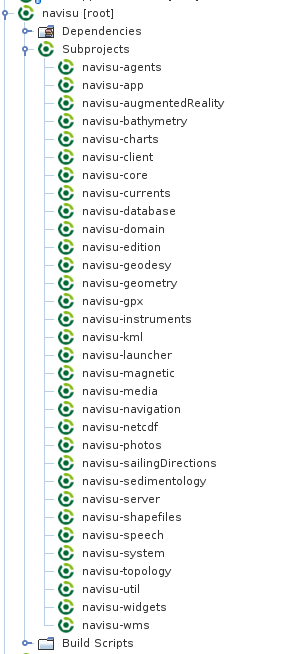
\includegraphics[height=20
 		cm]{images/architecture.png}
 	}
 	\begin{figure}[ht]
 		\caption{\label{3}\textit{Les modules de NaVisu}}
 	\end{figure}
 \end{center}
 %%%%%%%%%%%%%%%%%%%%%%%%%%%%%%%%%%%%%%%%%%%%%%%%%%%%%%%%%%%%%%%%%%%%%%%
 \newpage
 \subsection{Description succinte  des modules}
 \begin{itemize}
\item {\tt	navisu-bathymetry	}\\
Module m�tier, permet la visualisation de la bathym�trie, depuis une base de donn�es PostGis,  des images raster ou des fichiers NetCDF (d�veloppement en cours).
\item {\tt	navisu-charts	}\\
Module m�tier, permet la visualisation des catalogues de cartes vectorielles ou raster, l'affichage des cartes raster KAP ou GeoTiff et des cartes vectorielles S57. Dans le cas de cartes vectorielles chaque objet S57 est instanci� sous la forme d'un objet Java  susceptible de poss�der un comportement.
\item {\tt	navisu-client}\\
Module technique, permet le lien entre NaVisu et le serveur de donn�es des capteurs NMEA, AIS, ... Utilise le framework {\tt Vert.x} : \href{http://vertx.io/}{\tt http://vertx.io/ }pour l'impl�mentation de divers protocoles de communication. Les donn�es en entr�e sont en {\tt xml}, les data sont d�finies par un sch�ma. Les donn�es sont tout d'abord pars�es � l'aide de l'API JAXB, puis diffus�es dans l'application sous forme d'�v�nements $C�$.
\item {\tt	navisu-core	}\\
Module technique,  assure le lien avec la biblioth�que WorldWind d�velopp�e par la NASA, \href{https://goworldwind.org/}{\tt https://goworldwind.org/}
\item {\tt	navisu-currents	}\\
Module m�tier, permet la visualisation des donn�es open data de courants du Shom et des donn�es au format NetCDF (en cours)
\item {\tt	navisu-database	}\\
Module technique, permet la connexion � la base embarqu�e Derby, aux bases ext�rieures via JDBC (MySQL, PostGis), � la base embarqu�e Neo4J. Ce module utilise l'ORM EclipseLink afin que les objets puissent �tre trait�s comme des entit�es au sens de JPA, par exemple : les Ship, permettant de mettre en base les diff�rents navires signal�s par AIS.
\item {\tt	navisu-domain	}\\
Module technique, regroupe l'ensemble des mod�les de donn�es utilis�es, avec une faible d�pendance vis � vis des autres modules, il est facilement exportable.
\item {\tt	navisu-geodesy	}\\
Module technique, utile pour les calculs de distances, cap, ... sur le g�o�de. Cette biblioth�que utilise les formules Thaddeus Vincenty : \\
 \href{http://www.ngs.noaa.gov/PUBS_LIB/inverse.pdf}{\tt http://www.ngs.noaa.gov/PUBS\_LIB/inverse.pdf}, impl�ment�es  \\
 par Mike Gavaghan : 
 \href{https://github.com/mgavaghan/geodesy}{\tt https://github.com/mgavaghan/geodesy}
\item {\tt	navisu-geometry	}\\
Module technique, impl�mentation des courbes de B�zier, affichage et lissage par moindres carr�s et d'objets 3D au format {\tt obj}.
\item {\tt	navisu-gpx	}\\
Module technique, lecture et affichage dynamique des trajets au format Gpx : \\
\href{http://www.topografix.com/gpx.asp}{\tt http://www.topografix.com/gpx.asp}
\item {\tt	navisu-instruments	}\\
Module m�tier, ensemble des instruments permettant la lecture des donn�es de navigation. Ces instruments sont d�velopp�s en JavaFX/FXML, avec un strict respect du pattern MVC. Les instruments sont con�us pour pouvoir �tre int�gr�s � un syst�me t�te haute, ils sont portables sur mobiles Android ou IOS.
\item {\tt	navisu-kml	}\\
Module technique, lecture et affichage des donn�es au format KML.
\item {\tt	navisu-launcher	}\\
Module technique, module d'initialisation des connexions entre composants, lancement et arr�t de l'application.
\item {\tt	navisu-magnetic	}\\
Module m�tier, affichage du mod�le de d�clinaison magn�tique de la NOAA : \\ 
\href{https://www.ngdc.noaa.gov/geomag/}{\tt https://www.ngdc.noaa.gov/geomag/}
\item {\tt	navisu-media	}\\
Module technique, diffusion de fichiers sons.
\item {\tt	navisu-navigation	}\\
Module m�tier, ensemble de fonctionnalit�s d'aide � la navigation, pr�paration des routes et simulation. Impl�mentation des comportements des agents "intelligents" : balisage, amers.
\item {\tt	navisu-netcdf	}\\
Module technique, lecture g�n�rique des fichiers NetCDF, ce module est utilis� par les autres modules m�tier, m�t�o, bathym�trie, ...
\item {\tt	navisu-photos	}\\
Module technique, affichage de photos et d�codage des fichiers au format {\tt exif}.
\item {\tt	navisu-sailingDirections	}\\
Module m�tier, visualisation et �dition des Instructions Nautiques du Shom, [module en cours].
\item {\tt	navisu-sedimentology	}\\
Module m�tier, visualisation des donn�es du shom au format Shapefile.
\item {\tt	navisu-server	}\\
Module technique, premier module de NaVisu, permet l'acquisition de donn�es depuis plusieurs sources, multiplexe ces donn�es et les parse. Le r�sultat est envoy� au[x] client[s] sous forme xml.
\item {\tt	navisu-shapefiles	}\\
Module technique, module  g�n�rique de lecture des fichiers ShapeFile.
\item {\tt	navisu-speech	}\\
Module technique, module de synth�se de parole.
\item {\tt	navisu-system	}\\
Module technique, permet de lancer la lecture de fichiers de donn�es de diff�rents formats .
\item {\tt	navisu-topology	}\\
Module technique, permet de faire localement les diff�rentes op�rations d'inclusion, d'intersection, ... en utilisant la biblioth�que JTS Topology Suite : \\
 \href{http://tsusiatsoftware.net/jts/main.html}{\tt http://tsusiatsoftware.net/jts/main.html}. Permet aussi la triangulation des surfaces par la m�thode de Delaunay et le partitionnement par diagrammes de V�rono� en utilisant la biblioth�que {\tt JDelaunay } \href{https://github.com/orbisgis/jdelaunay}{\tt https://github.com/orbisgis/jdelaunay}
\item {\tt	navisu-widgets	}\\
Module technique, offre les services n�cessaires � la cr�ation et la manipulation des instruments.
\item {\tt	navisu-wms	}\\
Module technique, offre les services g�n�riques de consultation des web services. 
 \end{itemize}
\newpage
  \section{Deuxi�me niveau de modularit� : les composants}
  A l'int�rieur des modules, on va trouver une architecture en composants, construite � l'aide la biblioth�que $C^3$ : \href{http://c3.capcaval.org/}{\tt http://c3.capcaval.org/}
  
   %%%%%%%%%%%%%%%%%%%%%%%%%%%%%%%%%%%%%%%%%%%%%%%%%%%%%%%%%%%%%%%%%%%%%%%
   \begin{center}
   	\framebox[1\width]{
   		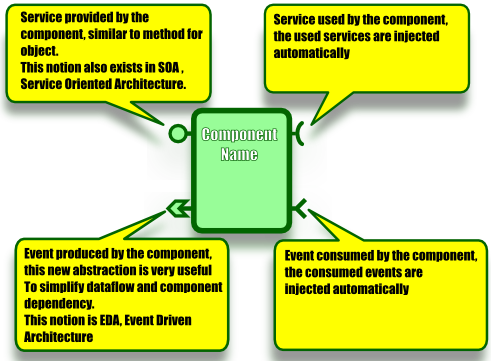
\includegraphics[height=11
   		cm]{images/component.png}
   	}
   	\begin{figure}[ht]
   		\caption{\label{3}\textit{Les E/S d'un composant }}
   	\end{figure}
   \end{center}
   %%%%%%%%%%%%%%%%%%%%%%%%%%%%%%%%%%%%%%%%%%%%%%%%%%%%%%%%%%%%%%%%%%%%%%%
   \subsection{Les services et les �v�nements}
   Comme pour les modules, on trouvera des composants techniques et des composants m�tier. Le composant est une abstraction qui permet de d�finir des services, � la fois rendus et consomm�s et des �v�nements � la fois rendus et consomm�s sans sp�cifier une impl�mentation particuli�re. L'impl�mentation est inject�e au d�marrage de l'application ainsi, si le contrat ou service est respect�, une modification de l'impl�mentation n'impactera pas l'ensemble de l'application, les modifications restant locales au composant. Les diff�rents composants de Navisu constituent l'architecture statique de l'application. Ensute selon les besoins ils instancierons  des contr�leurs pour 
   supporter la dynamique de l'application.
   
   \subsection{Application}
   Dans la pratique un composant est repr�sent� par deux interfaces et une classe d'impl�mentation. Il peut aussi instancier d'autres objets, comme des contr�leurs par exemple. l'ensemble du code ne va utiliser que son interface de service. Au d�marrage la biblioth�que $C�$ va injecter l'impl�mentation en cours.
   \subsection{Un exemple : le {\tt GpsLogger}}
   \begin{itemize}
   	\item {\bf Interface du composant} : Cette interface est tr�s simple, elle est une interface de typage pour la lib $C�$.
   	
\vspace{0.2cm}
   	\begin{boxedverbatim}
   	public interface GpsLogger	extends Component {
   	
   	}
   		\end{boxedverbatim}
   
   \vspace{0.5cm}
   	\item {\bf Interface des services} : 
   	
   	\vspace{0.2cm}
  	\begin{boxedverbatim} 
   public interface GpsLoggerServices extends ComponentService {
   
   void on(String ... files);
   
   default void off() {
   }
   
   boolean isOn();
   
   boolean canOpen(String category);
   
   InstrumentDriver getDriver();
   }
   
   		\end{boxedverbatim}
   		
   		 \vspace{0.5cm}
   	L'interface {\tt ComponentService} va apporter des contraintes techniques pour la gestion du cycle de vie du composant. Les autres services sont des services techniques : 
   	\begin{verbatim}
   boolean canOpen(String category);
   	\end{verbatim}
   	Permet � l'application de savoir si ce composant r�pond au crit�re demand� via le menu.
   		\begin{verbatim}
   		 InstrumentDriver getDriver();
   		\end{verbatim}
   		Retourne le composant pour action.\\
   		Ou sont des services m�tier : 
   		\begin{verbatim}
   		void on(String ... files);
   		\end{verbatim}
   		Met en route le Logger avec en argument z�ro ou des fichiers NMEA
   		\begin{verbatim}
   		default void off() {
   		}
   		\end{verbatim}
   		Arrete le service
   		\begin{verbatim}
   		boolean isOn();
   		\end{verbatim}
   		
   		Indique l'�tat du  service.\\
   	
\newpage
   \item {\bf Impl�mentation} : \\
   	\begin{boxedverbatim} 
   	public class GpsLoggerImpl
   	implements GpsLogger, GpsLoggerServices, 
   	                  InstrumentDriver, ComponentState {
   	
   	protected boolean on = false;
   	private final String NAME = "GpsLogger";
   	private GpsEventsController gpsEventsController;
   	
   	@Override
   	public void componentInitiated() {
   	}
   	@Override
   	public void componentStarted() {
   	}
   	@Override
   	public void componentStopped() {
   	}
   	@Override
   	public void on(String... files) {
     	if (on == false) {
    	on = true;
    	gpsEventsController = new GpsLoggerGpsEventsController();
    	gpsEventsController.subscribe();
   	   }
   	}
   	@Override
   	public void off() {
    	if (on == true) {
    	on = false;
    	}
   	}
   	@Override
   	public InstrumentDriver getDriver() {
    	return this;
   	}
   	@Override
   	public boolean canOpen(String category) {
    	return category.equals(NAME);
   	}
   	@Override
   	public boolean isOn() {
    	return on;
    	}
   	}
   \end{boxedverbatim} 
   
   	\newpage
   	\item {\bf Connexion et mise service du composant}, dans la classe {\tt AppMain} du module {\tt navisu-launcher} :
   	\begin{itemize}
   		\item D�claration de la classe d'impl�mentation 
   		\item Enregistrement du service aupr�s du componentManager
   		\item Enfin, puisqu'il sagit d'un composant qui sera activ� par le menu, enregistrement aupr�s de l'instrumentDriverManagerServices.
   	\end{itemize}
   	
   	Voir � ce propos le chapitre sur la cr�ation d'items de menu dans le dock.\\
   	\vspace{0.2cm}
   	
   		\begin{boxedverbatim} 
   LOGGER.info("\n"
   + componentManager.startApplication(
       
       ....
       
      GpsLoggerImpl.class,
       ....
     )
   );
   .....
   
   GpsLoggerServices gpsLoggerServices 
            = componentManager.getComponentService(GpsLoggerServices.class);
   
   .....
   
   instrumentDriverManagerServices.registerNewDriver(
                                  gpsLoggerServices.getDriver()
                            );
   
   	\end{boxedverbatim} 
   \end{itemize}
   
   \subsection{Les annotations}
   Nous avons vu pr�c�demment que l'interconnexion entre les composants se faisait � l'ex�cution, � la fois pour les services et les �v�nements. Les sp�cifications s'�crivent � l'aide des annotations.
   \begin{itemize}
   	\item Consommation d'un service : 
   	
   	 \vspace{0.2cm}
   	 \begin{boxedverbatim}
   	@UsedService
   	GuiAgentServices guiAgentServices;
   	 \end{boxedverbatim}
   	 
   	 \vspace{0.2cm}
   	 Un composant peut demander � consommer les services d'un autre composant. A partir de l� ce composant a acc�s aux services public du composant producteur.
   	 
   	 \vspace{0.2cm}
   	 \begin{boxedverbatim}
   	guiAgentServices.getRoot().getChildren().add(routeDataEditorController);
   	 \end{boxedverbatim}
   	 
   	 \vspace{0.2cm}
   	\newpage
   	\item Production d'un �v�nement
   	
   	\begin{itemize}
   		\item d�finition du mod�le de donn�e � transmettre :
   		
   		\vspace{0.2cm}
   		\begin{boxedverbatim}
   		public class Bathymetry {
   			
   			private List<Point3D> grid;
   			
   			public Bathymetry() {
   				  grid = new ArrayList<>();
   			}
   			public Bathymetry(List<Point3D> grid) {
   			 	 this.grid = grid;
   			}
   			public List<Point3D> getGrid() {
   			  	return grid;
   			}
   			public void setGrid(List<Point3D> grid) {
   			  	this.grid = grid;
   			}
   			public void add(Point3D point) {
   			    grid.add(point);
   			}
   			public int size() {
   				 return grid.size();
   			}
   			@Override
   			public String toString() {
   				 return "Bathymetry{" + "grid=" + grid + '}';
   			}
   		}
   		\end{boxedverbatim}
   		\vspace{0.2cm}
   		\item D�finition de l'interface de l'�v�nement
   		
   		\vspace{0.2cm}
   		\begin{boxedverbatim}
   		public interface BathymetryEvent
   		extends ComponentEvent {
   			
   			public void notifyBathymetryMessageChanged(Bathymetry data);
   		}
   		\end{boxedverbatim}
   		
   		\vspace{0.2cm}
   		
   		\item D�finition de l'interface de services de tir
   		
   		\vspace{0.2cm}
   		\begin{boxedverbatim}
   			public interface BathymetryEventProducerServices
   			extends ComponentService {
   				
   				public void setBathymetry(Bathymetry data);
   				
   			}
   		\end{boxedverbatim}
   		
   	\newpage
   		\item L'impl�mentation d'un tireur d'�v�nement 
   		
   		\vspace{0.2cm}
   			\begin{boxedverbatim}
   				public class BathymetryEventProducerImpl
   				implements BathymetryEventProducer, 
   				BathymetryEventProducerServices {
   					
   					@ProducedEvent
   					protected BathymetryEvent bathymetryEvent;
   					
   					@Override
   					public void setBathymetry(Bathymetry evt) {
   					          	bathymetryEvent.notifyBathymetryMessageChanged(evt);
   					}
   					
   			}
   			\end{boxedverbatim}
   			
   			\vspace{0.2cm}
   			\item Le tir
   			
   			\vspace{0.2cm}
   			\begin{boxedverbatim}
   			bathymetryEventProducerServices.setBathymetry(new Bathymetry(data));
   			\end{boxedverbatim}
   	\end{itemize}
   
   	
   	\item Consommation d'un �v�nement
   	
   	\begin{itemize}
   		\item D�claration d'int�r�t
   
   	
   	\vspace{0.2cm}
   	\begin{boxedverbatim}
   	ComponentManager cm = ComponentManager.componentManager;
   	ComponentEventSubscribe<BathymetryEvent> bathyES =
                	 cm.getComponentEventSubscribe(BathymetryEvent.class);
   	
   	\end{boxedverbatim}
   	
   	\vspace{0.2cm}
   	\item Impl�mentation de l'interface correspondant � l'�v�nement : 
   	
   		\vspace{0.2cm}
   	\begin{boxedverbatim}
   	private void subscribe() {
   		bathyES.subscribe(new BathymetryEvent() {
   			
   			@Override
   			public void notifyBathymetryMessageChanged(Bathymetry data) {
   				if (data.size() != 0) {
   				 	// logique applicative
   				 }
   				});
   			}
   	\end{boxedverbatim}
   		\end{itemize}
   \end{itemize}
   
   	\vspace{0.2cm}
   	
   	Et voil� 	
\includegraphics[height=1cm]{images/presence_offline.png} \\
   	
   	Avec cette architecture, le producteur ne connait pas le ou les consommateurs, les consommateurs n'ont pas de connaissance directe du producteur, ils connaissent simplement un service. A noter que le producteur doit �tre un composant, par contre une simple classe peut aussi �tre une consommatrice d'�v�nements.
   	
   	
%\chapter{Architecture et fonctionnalit�s du serveur de donn�es}


\section{Pr�sentation}

Le module d'acquisition de donn�es de \nav\  est distribu�. Un serveur re�oit les donn�es des diff�rents capteurs
les analyse, les traite puis les distribue au format XML [ou JSON (option)] aux diff�rents clients. Dans la version la plus compacte serveur et client se trouvent sur une m�me machine.
 Le protocole de communication utilis� sont les WebSockets. \footnote{\href{http://fr.wikipedia.org/wiki/WebSocket}{http://fr.wikipedia.org/wiki/WebSocket}} ce protocole permet les actions bidirectionnelles, {\em push} et {\em pull}, avec les clients. Actuellement seules les requ�tes {\em pull} venant des clients sont prises en compte, mais il est simple d'introduire des actions {\em push} de la part du serveur pour des remont�es d'alarmes par exemple.
 Le protocole WebSocket est impl�ment� dans la plupart des langages actuellement.
 L'impl�mentation du serveur repose sur le {\em framework } Vert.x \footnote{\href{http://vertx.io/}{http://vertx.io/}}
 \footnote{\href{http://fr.wikipedia.org/wiki/Vert.x}{http://fr.wikipedia.org/wiki/Vert.x}}, ce {\em framework} assure la communication asynchrone entre les entr�es et les sorties du serveur, � l'aide de bus �v�nementiels : {\tt EventBus}.
 Il est simple � utiliser, ne n�cessite pas d'installation particuli�re. 
 L'int�r�t de la distribution est la possibilit� des d�velopper des clients ayant 
 diff�rentes technologies d'interfaces : JavaFX, HTML5 et diff�rents OS : Windows7/Windows8, Mac OS, iOS, Linux ou Android. les clients peuvent �tre une application \nav\ compl�te ou de simple affichages de donn�es capteurs : des instruments par exemple, ou des clients de communication type chat.
 
 %%%%%%%%%%%%%%%%%%%%%%%%%%%%%%%%%%%%%%%%%%%%%%%%%%%%%%%%%%%%%%%%%%%%%%%
 \begin{center}
 \framebox[1\width]{
 	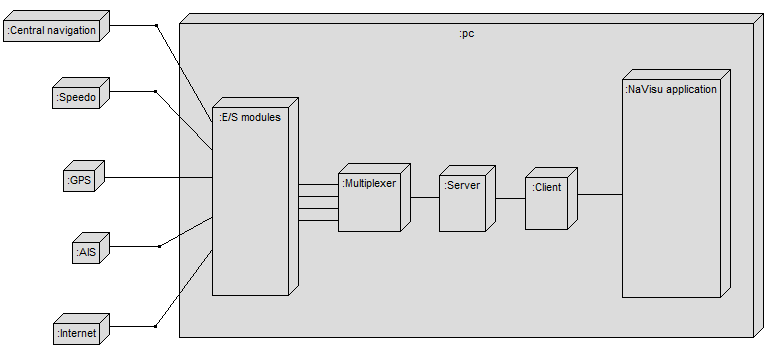
\includegraphics[width=16cm,height=10cm]{images/dataserver/deploiement_0.png}
 }
 \begin{figure}[ht]
 \caption{\label{3}\textit{D�ploiement centralis�}}
 \end{figure}
 \end{center}
 %%%%%%%%%%%%%%%%%%%%%%%%%%%%%%%%%%%%%%%%%%%%%%%%%%%%%%%%%%%%%%%%%%%%%%%
 \begin{center}
 \framebox[1\width]{
 	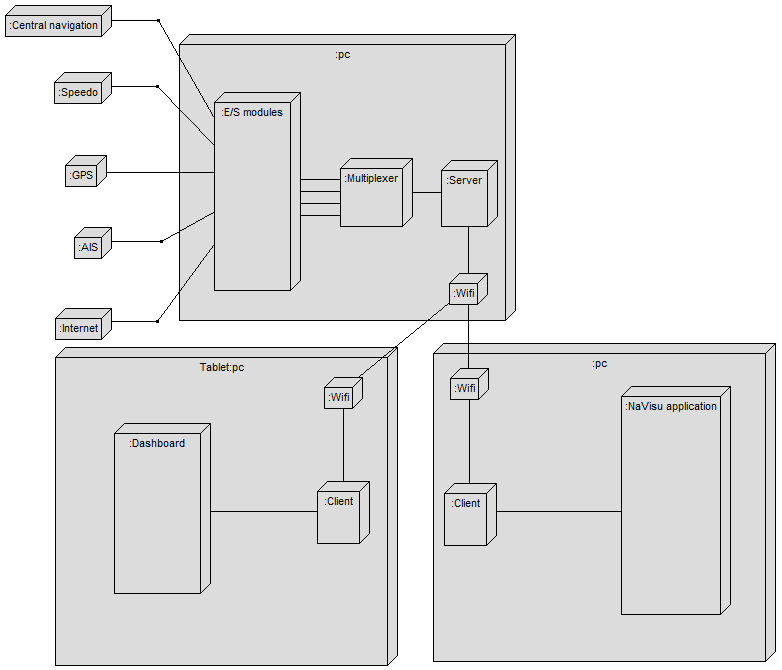
\includegraphics[width=16cm,height=10cm]{images/dataserver/deploiement_1.png}
 }
 \begin{figure}[ht]
 \caption{\label{3}\textit{D�ploiement distribu�}}
 \end{figure}
 \end{center}

 \section{Les donn�es en entr�e}
 Les donn�es sont envoy�es au serveur via les ports s�rie, USB ou Internet.
 Il est aussi possible d'avoir des donn�es � partir de fichiers, pour un rejeu de parcours par exemple.
 L'acquisition de donn�es est r�alis�e par des objets {\bf\tt Reader}, 
 \begin{center}
   \begin{minipage}{16cm}
   \begin{itemize}
   \item {\bf\tt SerialReader} pour la communication s�rie
   \item {\bf\tt HTTPReader} pour la saisie sur internet
   \item {\bf\tt FileReader} pour la lecture de donn�es sur disque
   \end{itemize}
   \end{minipage}
 \end{center}  
  Le composant {\bf\tt DataServer} peut cr�er en dynamique les diff�rents {\bf\tt Reader} et les param�trer.
  Exemples de  d�bits sur les ports s�rie : 
  \begin{center}
  \begin{minipage}{16cm}
  \begin{itemize}
  \item 4800 bauds (GPS, centrale de navigation, \ldots, NMEA0183 ASCII)
  \item 38400 bauds (AIS, NMEA0183 binaire)
  \item 250 Kbits/sec (GPS, centrale de navigation, moteurs, \ldots,N2K binaire)
  \end{itemize}
  \end{minipage}
  \end{center} 
   Exemples de  frames pour les entr�es capteurs :
    {\small
    \begin{verbatim}
 NMEA0183  : $GPRMC,093518.470,A,4826.2552,N,00429.8708,W,000.0,203.5,051113,,,A*7A
 AIS       : !AIVDM,1,1,,B,13IMVT0000OcEt8KcIfW75F@0<0>,0*52
 NMEA 2000 : <0x18eeff01> [8] 05 a0 be 1c 00 a0 a0 c0
    \end{verbatim}
    }
\section{L'architecture}\footnote{Dans les figures qui suivent les flux de donn�es dynamiques sont colori�s en turquoise, les canaux de communication en gris clair.}

%%%%%%%%%%%%%%%%%%%%%%%%%%%%%%%%%%%%%%%%%%%%%%%%%%%%%%%%%%%%%%%%%%%%%%%
\begin{center}
\framebox[1\width]{
	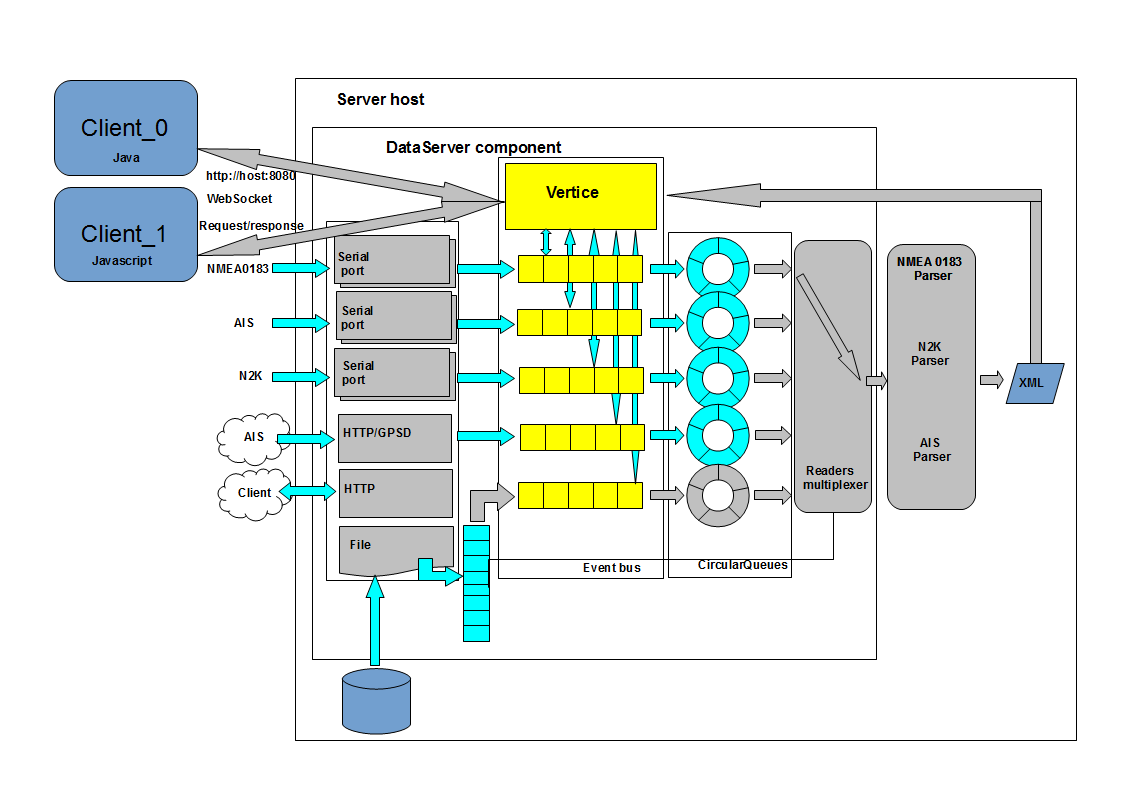
\includegraphics[width=16cm,height=12cm]{images/dataserver/dataServer_0.png}
	}
\begin{figure}[ht]	
\caption{\label{1}\textit{Aucune requ�te client, les donn�es dynamiques venant des capteurs sont perdues}}
\end{figure}
\end{center}
%%%%%%%%%%%%%%%%%%%%%%%%%%%%%%%%%%%%%%%%%%%%%%%%%%%%%%%%%%%%%%%%%%%%%%%
Un {\bf\tt Reader} sp�cialis� est associ� � chaque entr�e, un bus d'�v�nements Vert.x lui est attribu�, ainsi
qu'une file circulaire.
En entr�e continu les donn�es sont envoy�es, via leur bus, � leur file. En sortie le d�bit d'acquisition  est pilot� par chaque client.Si il n'y a pas de requ�tes client, les
nouvelles donn�es �crasent les anciennes, sauf pour celles venant de fichiers qui sont transf�r�es int�gralement.
Un s�lecteur de {\bf\tt Reader} assure le multiplexage des donn�es, actuellement la strat�gie du choix est simple parcours circulaire, mais une strat�gie avec file � priorit� peut �tre facilement mise en \oe uvre. Sur requ�te d'un client
la file circulaire active d�livre ses donn�es au s�lecteur d'analyseur syntaxique: NMEA0183, AIS, N2K. 
Le parseur choisi traite les donn�es, g�n�re des objets NMEA, les transforme au format XML et les envoie � l'objet {\bf\tt Vertice} qui les envoie au client. Une nouvelle file est s�lectionn�e dans l'attente d'une autre requ�te client.
Les donn�es sont donc analys�es ({\em pars�es}) deux fois, une premi�re fois par le parseur NMEA sp�cialis�, une deuxi�me fois par le client � partir de d'un format XML. Ceci se justifie par le fait que l'�criture du premier parseur est complexe du fait de la grande variabilit� des formats NMEA, les connexions �lectriques avec les capteurs peuvent aussi engendrer  
un bruitage des donn�es, ces donn�es sont ensuite mises en forme suivant un sch�ma XML unique, les clients n'ont aucune difficult�s � les transformer en objets � partir de l'API JAXB. D�s que le format JSON sera bien int�gr� � JEE, ce
format sera pr�f�r� � XML. D'autres protocoles, tel que CoAP sont envisageables dans l'avenir.
\section{La dynamique}
%%%%%%%%%%%%%%%%%%%%%%%%%%%%%%%%%%%%%%%%%%%%%%%%%%%%%%%%%%%%%%%%%%%%%%%
\begin{center}
\framebox[1\width]{
	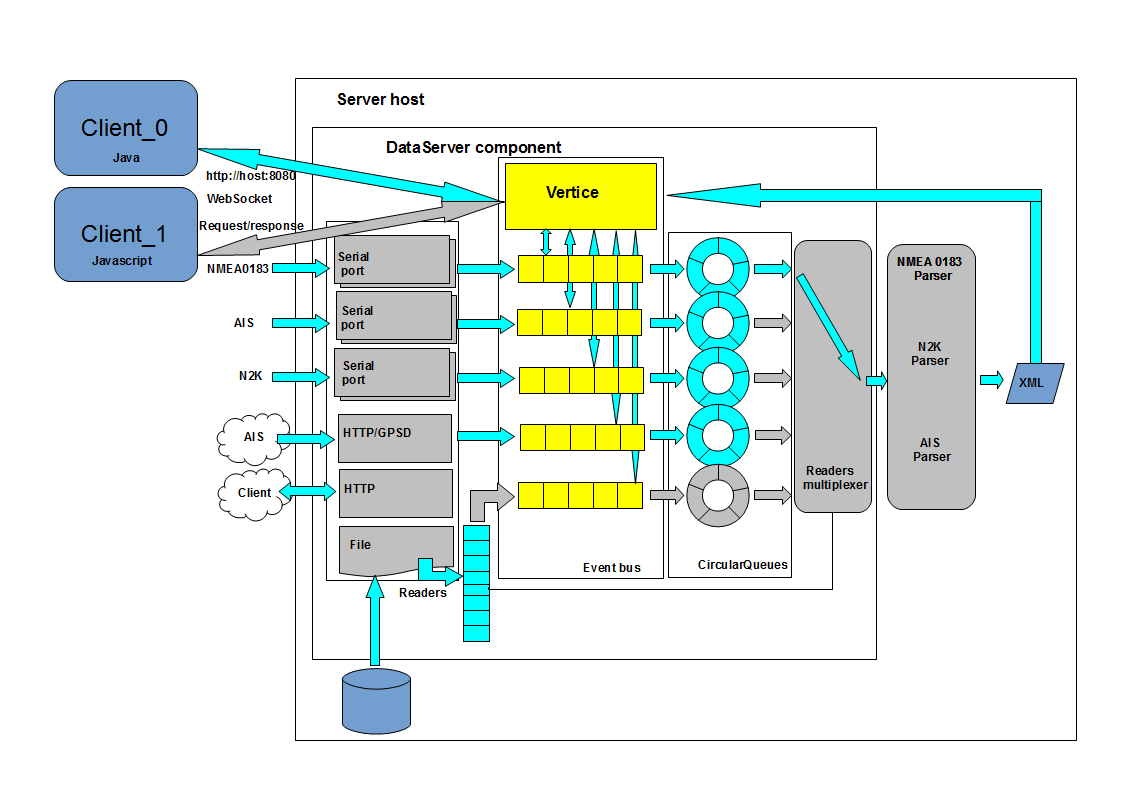
\includegraphics[width=16cm,height=12cm]{images/dataserver/dataServer_1.png}
}
\begin{figure}[ht]
\caption{\label{2}\textit{Exemple de requ�te client, suivie d'une r�ponse asynchrone � partir du premier port s�rie enregistr�.}}
\end{figure}
\end{center}

\subsection{Performances}
En test, le serveur supporte une requ�te client toutes les milisecondes, dans la pratique, un navire naviguant � 15 n\oe uds 
parcourt 7.5m en une seconde, un barreur va r�gler le d�bit d'affichage des donn�es � 2 ou 3 secondes. Une p�riode de 
1 seconde pour les requ�tes semble raisonnable.
%%%%%%%%%%%%%%%%%%%%%%%%%%%%%%%%%%%%%%%%%%%%%%%%%%%%%%%%%%%%%%%%%%%%%%%
\begin{center}
\framebox[1\width]{
	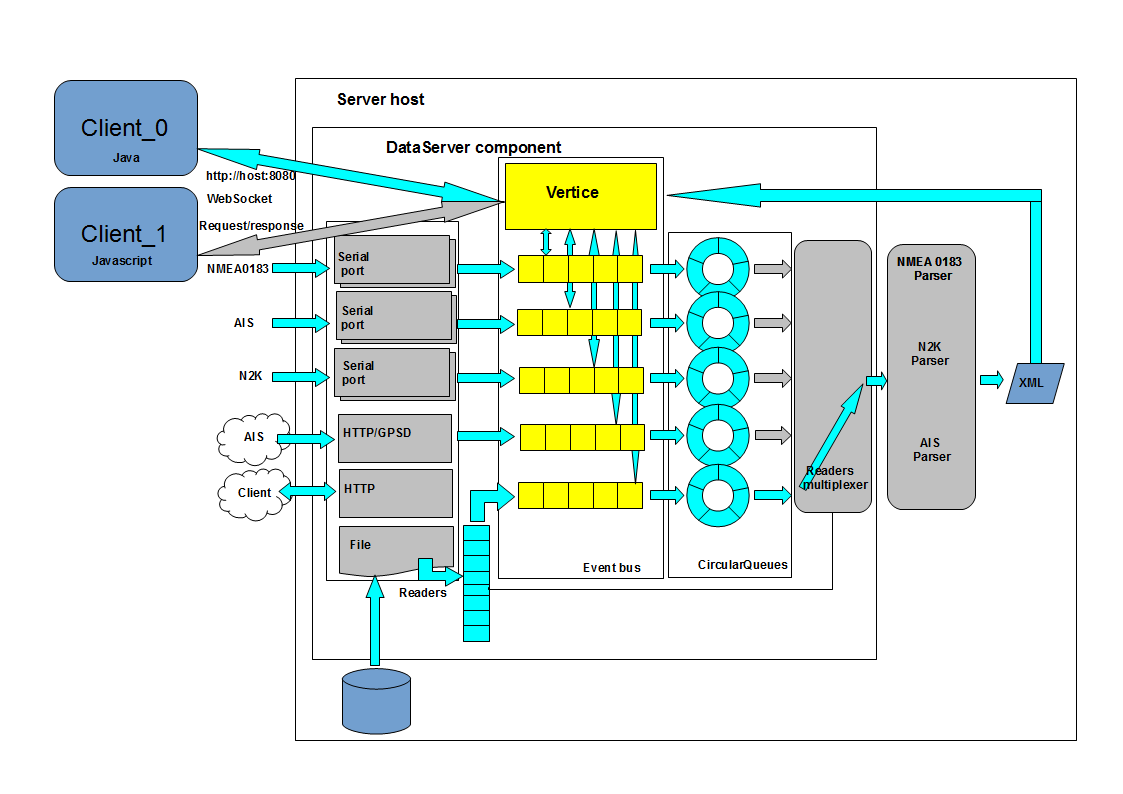
\includegraphics[width=16cm,height=12cm]{images/dataserver/dataServer_2.png}
}
\begin{figure}[ht]
\caption{\label{3}\textit{Exemple de requ�te client, suivie d'une r�ponse synchrone � partir de donn�es provenant d'un fichier.}}
\end{figure}
\end{center}
%%%%%%%%%%%%%%%%%%%%%%%%%%%%%%%%%%%%%%%%%%%%%%%%%%%%%%%%%%%%%%%%%%%%%%%
\section{Les donn�es en sortie (extrait)}
{\small
 \begin{verbatim}
<?xml version="1.0" encoding="UTF-8" standalone="true"?>
-<sentences>
-<rmc>
  <device>GP</device>
  <sentence>
    $GPRMC,191137.304,A,4826.2620,N,00429.8665,W,000.0,225.3,050114,,,A*7C
  </sentence>
  <eastOrWestVariation/>
  <date>2014-01-05T19:11:37.972+01:00</date>
  <status>A</status>
  <latitude>48.437702</latitude>
  <longitude>-4.4977746</longitude>
  <variation>0.0</variation>
  <track>225.3</track>
  <sog>0.0</sog>
</rmc>
-<gga>
  <device>GP</device>
  <sentence>
    $GPGGA,191138.000,4826.2632,N,00429.8614,W,2,05,1.2,72.4,M,52.1,M,0.8,0000*50
  </sentence>
  <utc>2014-01-05T19:11:38.973+01:00</utc>
  <latitude>48.43772</latitude>
  <longitude>-4.4976897</longitude>
  <gpsQualityIndicator>2</gpsQualityIndicator>
  <numberOfSatellitesInView>5</numberOfSatellitesInView>
  <horizontalDilutionOfPrecision>1.2</horizontalDilutionOfPrecision>
  <antennaAltitude>72.4</antennaAltitude>
  <unitsOfAntennaAltitude>M</unitsOfAntennaAltitude>
  <geoidAltitude>52.1</geoidAltitude>
  <unitsOfGeoidAltitude>M</unitsOfGeoidAltitude>
  </gga>
</sentences>
\end{verbatim}
}

%\chapter{Les donn�es NMEA 0183}

%Ref : TV080114\_TU\_SM \hfill R�dacteur : Serge  Morvan \\



\section{Le standard NMEA}
http://standards.nmea.org/
Le site officiel : \\
 \hbox{}\hspace{1cm}\href{http://www.nmea.org/}{http://www.nmea.org/} \\
 Des informations sur le contenu des phrases : \\
 \hbox{}\hspace{1cm}\href{http://gpsinformation.net/}{http://gpsinformation.net/}\\
 \hbox{}\hspace{1cm}\href{http://gpsd.berlios.de/NMEA.html}{http://gpsd.berlios.de/NMEA.html}\\
 \hbox{}\hspace{1cm}\href{http://www.kh-gps.de/nmea.faq}{http://www.kh-gps.de/nmea.faq}\\
 Un projet de service d�mon :\\
 \hbox{}\hspace{1cm}\href{http://catb.org/gpsd/}{http://catb.org/gpsd/}\\

\newpage
\section{Mod�le NMEA0183}
\subsection{Ensemble des phrases analys�es}
\begin{center}
\framebox[1\width]{
	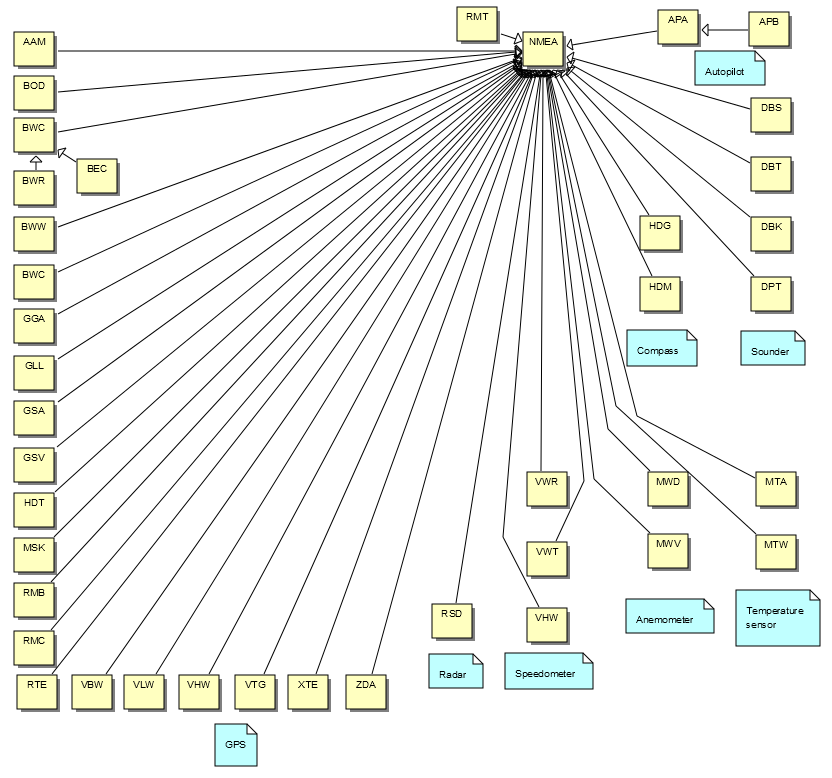
\includegraphics[width=18cm]{images/nmea/nmea.png}
}
\begin{figure}[h]
\caption{\label{nmea}\textit{Ensemble des classes de l'API NMEA}}
\end{figure}
\end{center}
%%%%%%%%%%%%%%%%%%%%%%%%%%%%%%%%%%%%%%%%%%%%%%%%%%%%%%%%%%%%%%%%%%%%%%%
%%%%%%%%%%%%%%%%%%%%%%%%%%%%%%%%%%%%%%%%%%%%%%%%%%%%%%%%%%%%%%%%%%%%%%
\begin{center}
\framebox[1\width]{
	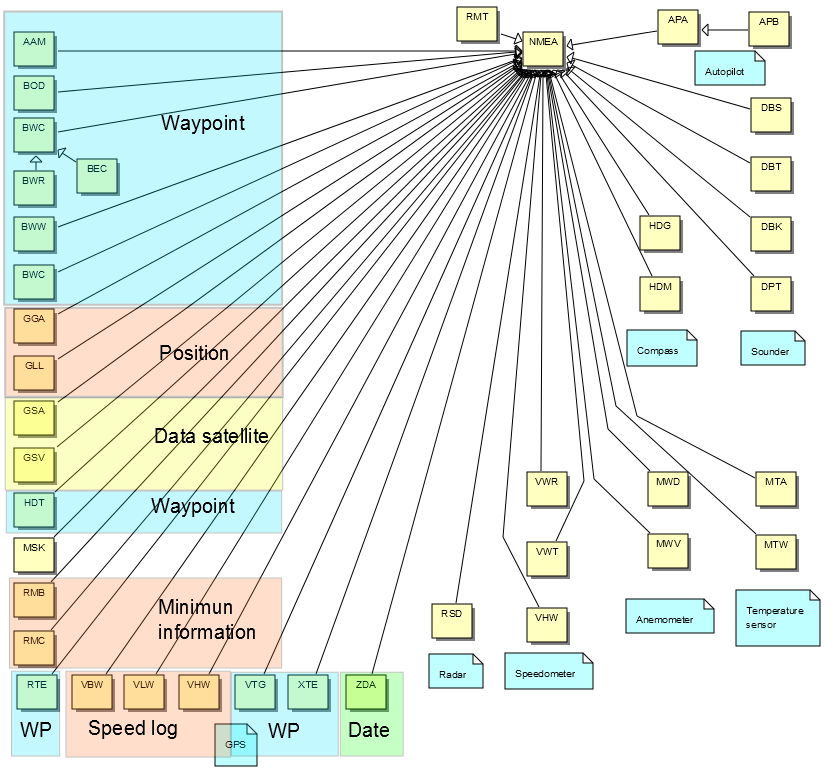
\includegraphics[width=17cm]{images/nmea/nmea_comment.png}
}
\begin{figure}[h]
\caption{\label{repart}\textit{Cat�gorisation des informations NMEA}}
\end{figure}
\end{center}
%%%%%%%%%%%%%%%%%%%%%%%%%%%%%%%%%%%%%%%%%%%%%%%%%%%%%%%%%%%%%%%%%%%%%%%
%%%%%%%%%%%%%%%%%%%%%%%%%%%%%%%%%%%%%%%%%%%%%%%%%%%%%%%%%%%%%%%%%%%%%%
\subsection{Minimun d'information pour la navigation}
\begin{center}
\framebox[1\width]{
	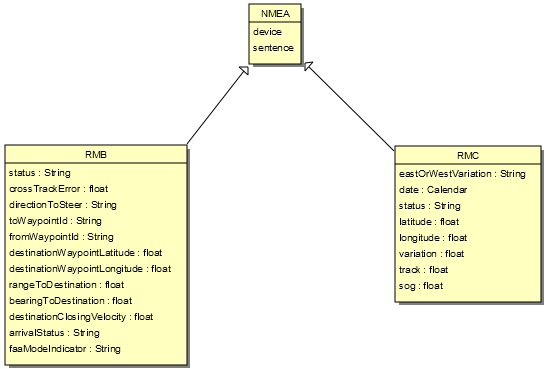
\includegraphics[width=16cm]{images/nmea/gps_minimum.png}
}
\begin{figure}[h]
\caption{\label{gpsminimum}\textit{Minimun d'information pour la navigation}}
\end{figure}
\end{center}
%%%%%%%%%%%%%%%%%%%%%%%%%%%%%%%%%%%%%%%%%%%%%%%%%%%%%%%%%%%%%%%%%%%%%%%
%%%%%%%%%%%%%%%%%%%%%%%%%%%%%%%%%%%%%%%%%%%%%%%%%%%%%%%%%%%%%%%%%%%%%%
\subsection{Date et heure}
\begin{center}
\framebox[1\width]{
	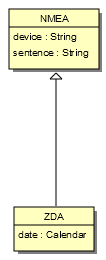
\includegraphics[width=3cm]{images/nmea/date.png}
}
\begin{figure}[h]
\caption{\label{date}\textit{Date}}
\end{figure}
\end{center}
%%%%%%%%%%%%%%%%%%%%%%%%%%%%%%%%%%%%%%%%%%%%%%%%%%%%%%%%%%%%%%%%%%%%%%%
%%%%%%%%%%%%%%%%%%%%%%%%%%%%%%%%%%%%%%%%%%%%%%%%%%%%%%%%%%%%%%%%%%%%%%
\subsection{Position : latitude, longitude}
\begin{center}
\framebox[1\width]{
	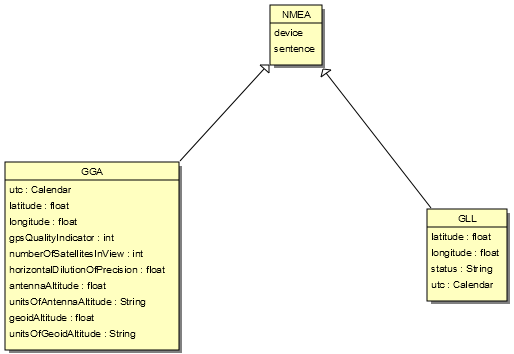
\includegraphics[width=16cm]{images/nmea/position.png}
}
\begin{figure}[h]
\caption{\label{position}\textit{Informations de position}}
\end{figure}
\end{center}
%%%%%%%%%%%%%%%%%%%%%%%%%%%%%%%%%%%%%%%%%%%%%%%%%%%%%%%%%%%%%%%%%%%%%%%
%%%%%%%%%%%%%%%%%%%%%%%%%%%%%%%%%%%%%%%%%%%%%%%%%%%%%%%%%%%%%%%%%%%%%%
\subsection{Informations de vitesse et de distance}
\begin{center}
\framebox[1\width]{
	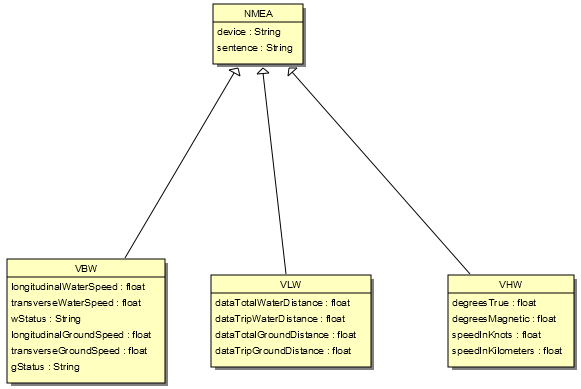
\includegraphics[width=16cm]{images/nmea/speedLog.png}
}
\begin{figure}[h]
\caption{\label{speedLog}\textit{Informations de vitesse et de distance}}
\end{figure}
\end{center}
%%%%%%%%%%%%%%%%%%%%%%%%%%%%%%%%%%%%%%%%%%%%%%%%%%%%%%%%%%%%%%%%%%%%%%%
%%%%%%%%%%%%%%%%%%%%%%%%%%%%%%%%%%%%%%%%%%%%%%%%%%%%%%%%%%%%%%%%%%%%%%
\subsection{Informations sur les waypoints}
\begin{center}
\framebox[1\width]{
	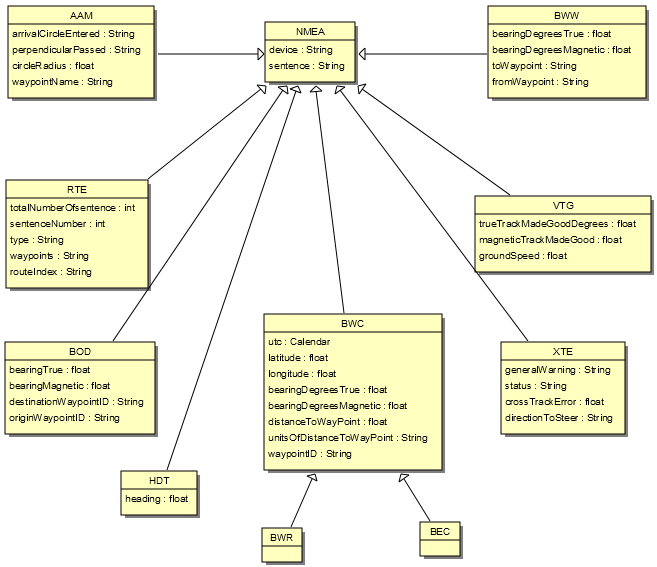
\includegraphics[width=16cm]{images/nmea/waypoint.png}
}
\begin{figure}[h]
\caption{\label{waypoint}\textit{Informations sur les waypoints}}
\end{figure}
\end{center}
%%%%%%%%%%%%%%%%%%%%%%%%%%%%%%%%%%%%%%%%%%%%%%%%%%%%%%%%%%%%%%%%%%%%%%%
%%%%%%%%%%%%%%%%%%%%%%%%%%%%%%%%%%%%%%%%%%%%%%%%%%%%%%%%%%%%%%%%%%%%%%
\subsection{Informations sur les satellites}
\begin{center}
\framebox[1\width]{
	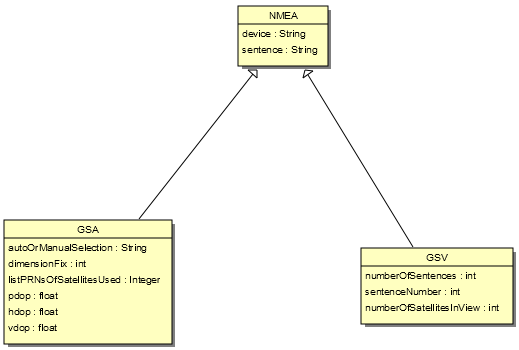
\includegraphics[width=16cm]{images/nmea/satellite.png}
}
\begin{figure}[h]
\caption{\label{satellite}\textit{Informations sur les satellites}}
\end{figure}
\end{center}

%%%%%%%%%%%%%%%%%%%%%%%%%%%%%%%%%%%%%%%%%%%%%%%%%%%%%%%%%%%%%%%%%%%%%%%
%%%%%%%%%%%%%%%%%%%%%%%%%%%%%%%%%%%%%%%%%%%%%%%%%%%%%%%%%%%%%%%%%%%%%%
\subsection{Informations sur le vent}
\begin{center}
\framebox[1\width]{
	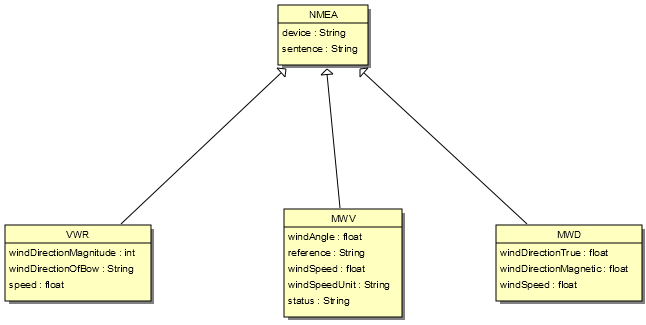
\includegraphics[width=16cm]{images/nmea/anemometer.png}
}
\begin{figure}[h]
\caption{\label{anemometer}\textit{Informations sur le vent}}
\end{figure}
\end{center}
%%%%%%%%%%%%%%%%%%%%%%%%%%%%%%%%%%%%%%%%%%%%%%%%%%%%%%%%%%%%%%%%%%%%%%%
%%%%%%%%%%%%%%%%%%%%%%%%%%%%%%%%%%%%%%%%%%%%%%%%%%%%%%%%%%%%%%%%%%%%%%
\subsection{Bathym�trie}
\begin{center}
\framebox[1\width]{
	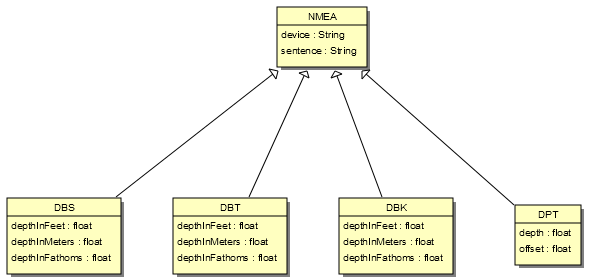
\includegraphics[width=16cm]{images/nmea/depth.png}
}
\begin{figure}[h]
\caption{\label{depth}\textit{Bathym�trie}}
\end{figure}
\end{center}
%%%%%%%%%%%%%%%%%%%%%%%%%%%%%%%%%%%%%%%%%%%%%%%%%%%%%%%%%%%%%%%%%%%%%%%

 %%%%%%%%%%%%%%%%%%%%%%%%%%%%%%%%%%%%%%%%%%%%%%%%%%%%%%%%%%%%%%%%%%%%%%
 \section{Pr�sentation de l'API}
 L'API permet l'acc�s au mod�le NMEA que nous avons choisit, celui-ci est proche
 de l'ensemble des phrases mais s'en �loigne parfois lorsqu'il y a redondance
 d'information dans une phrase, plusieurs valeurs de vitesse dans diff�rentes
 unit�s par exemple, ou lorsqu'une structure plus �labor�e permet de stocker des
 donn�es : liste, dictionnaire, \ldots
 \subsection{L'analyseur lexical et syntaxique}
 Le standard NMEA a beaucoup �volu�, plusieurs constructeurs ont impos� leur
 modifications, ce qui fait que de nombreuses variantes apparaissent dans les
 sorties NMEA des diff�rents appareils. Nous avons choisi d'uiliser le g�n�rateur
 d'analyseurs lexicaux et syntaxiques ANTLR pour plus de clart� du code. \\
 \hbox{}\hspace{1cm}\href{http://www.antlr.org/}{http://www.antlr.org/} \\
 \newpage
 En plus de cet outil nous utilisons l'atelier ANTLRWorks : \\ 
 \hbox{}\hspace{1cm}\href{http://www.antlr.org/works/}{http://www.antlr.org/works/}
 \\ Cet atelier permet de visualiser les grammaires cr��es.
 \subsubsection{Un exemple simple} 
 \small
 \begin{verbatim}
 GSV	     : '$' device=DEVICE 'GSV' 
 (NUMBER | SEP)+ 
 checksum=CHECKSUM
 { //action }
 \end{verbatim}
 \normalsize{}
 \begin{center}
 	\framebox[1\width]{
 		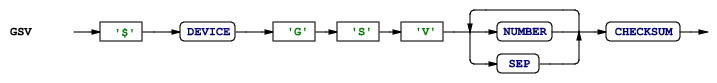
\includegraphics[width=12cm]{images/nmea/gsv.png}
 	}
 	\begin{figure}[h]
 		\caption{\label{gsv}\textit{Analyse de la phrase GSV}}
 	\end{figure}
 \end{center}
 
 \subsubsection{Un exemple plus complexe}
 \small
 \begin{verbatim}
 RMB     : '$' device = DEVICE 'RMB' SEP 
 status = LETTERS SEP  
 (crossTrackError =  NUMBER)* SEP
 (directionToSteer = LETTERS)* SEP
 (fromWaypointId = LETTERS |fromWaypointId = NUMBER)*  SEP
 (toWaypointId =  LETTERS | toWaypointId = NUMBER)* SEP
 (destinationWaypointLatitude =  NUMBER)* SEP (ns = LETTERS)* SEP
 (destinationWaypointLongitude  =  NUMBER)* SEP (ew  = LETTERS)* SEP
 (rangeToDestination =  NUMBER)* SEP
 (bearingToDestination =  NUMBER)* SEP
 (destinationClosingVelocity =  NUMBER)* SEP 	        	    
 (LETTERS SEP)*
 (arrivalStatus = LETTERS | '\u0000')* 
 checksum=CHECKSUM 
 { // action}
 \end{verbatim}
 \normalsize{}
 \begin{center}
 	\framebox[1\width]{
 		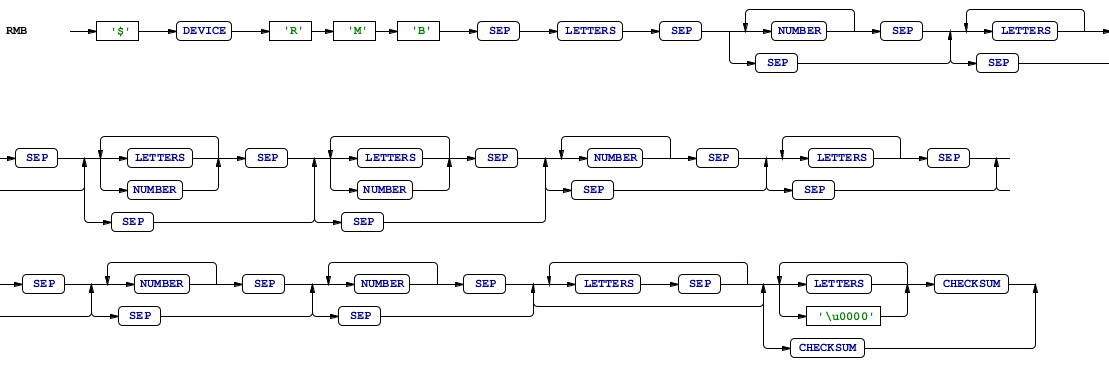
\includegraphics[width=12cm]{images/nmea/rmb.png}
 	}
 	\begin{figure}[h]
 		\caption{\label{dbt}\textit{Analyse de la phrase RMB}}
 	\end{figure}
 \end{center}
 
 %%%%%%%%%%%%%%%%%%%%%%%%%%%%%%%%%%%%%%%%%%%%%%%%%%%%%%%%%%%%%%%%%%%%%%

%%%%%%%%%%%%%%%%%%%%%%%%%%%%%%%%%%%%%%%%%%%%%%%%%%%%%%%%%%%%%%%%%%%%%%%

\section{Glossaire}
\begin{tabular}{|l|l|l|}
\hline
\bf Acronyme & \bf Expansion \\
\hline
AAM & Waypoint Arrival Alarm  \\
\hline
ALM & GPS Almanac Data \\
\hline
APA & Autopilot Sentence ``A''\\
\hline
APB  & Autopilot Sentence ``b''\\
\hline
BEC & Bearing and Distance to Waypoint,  Dead Reckoning\\
\hline
BOD & Bearing, Waypoint to Waypoint\\
\hline
BWC & Bearing and Distance to Waypoint\\
\hline
BWR  & Bearing and Distance to Waypoint   \\
\hline
BWW & Bearing and  Waypoint to Waypoint \\
\hline
DBK & Depth Below Keel \\
\hline
DBS & Depth Below Surface \\
\hline
DBT & Depth Below Transducer \\
\hline
DPT & Depth and offset \\
\hline
GGA &  Global Positioning System Fix Data. Time \\
\hline
GLL & Geographic Position and Latitude/Longitude \\
\hline
GSA & GPS DOP and active satellites \\
\hline
GSV & Satellites in view \\
\hline
GTD & Geographic Location in Time Differences \\
\hline
HDG & Heading, Deviation and Variation \\
\hline
HDM & Heading Magnetic \\
\hline
HDT & Heading True \\
\hline
MTW & Water Temperature \\
\hline
MWV & Wind Speed and Angle \\
\hline
RMA & Recommended Minimum Navigation Information \\
\hline
RMB & Recommended Minimum Navigation Information \\
\hline
RMC & Recommended Minimum Navigation Information \\
\hline
RTE & Routes \\
\hline
VBW & Dual Ground/Water Speed \\
\hline
VHW & Water Speed and Heading \\
\hline
VLW & Distance Traveled through Water \\
\hline
VPW & Speed, Measured Parallel to Wind \\
\hline
VTG & Track Made Good and Ground Speed \\
\hline
VWR & Relative Wind Speed and Angle \\
\hline
XTE & Cross-Track Error  Measured \\
\hline
ZDA & Time, Date and UTC, Day, Month, Year and Local Time Zone \\
\hline
\end{tabular}


%\chapter{Architecture et fonctionnalit�s du client NMEA}

%Ref : TV240114\_TU\_SM \hfill R�dacteur : Serge  Morvan \\


\section{Les connexions au serveur}
Les diff�rents p�riph�riques et capteurs fournissent les donn�es de navigation au serveur, suivant diff�rents
protocoles. Ces donn�es sont multiplex�es par le serveur. Sur requ�te des clients elles sont analys�es, transform�es dans un format XML standard et envoy�es aux diff�rents clients. Ces clients peuvent �tre sur la m�me machine dans
le cas le plus simple ou sur d'autres ordinateurs, tablettes ou smartphones. \nav\ est le client le plus riche.
%%%%%%%%%%%%%%%%%%%%%%%%%%%%%%%%%%%%%%%%%%%%%%%%%%%%%%%%%%%%%%%%%%%%%%%
\begin{center}
\framebox[1\width]{
	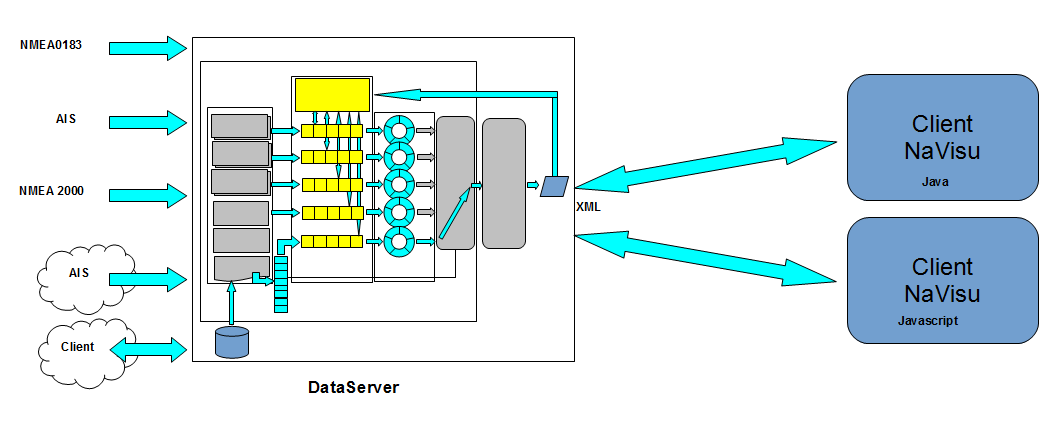
\includegraphics[width=16cm]{images/dataServer_3.png}
}
\begin{figure}[ht]
\caption{\label{0}\textit{Sch�ma g�n�ral des entr�es/sorties}}
\end{figure}
\end{center}
%%%%%%%%%%%%%%%%%%%%%%%%%%%%%%%%%%%%%%%%%%%%%%%%%%%%%%%%%%%%%%%%%%%%%%%
\section{Les donn�es en entr�e}
Il n'existe pas, � notre connaissance, de sch�ma XML bien d�fini pour l'ensemble des donn�es NMEA.
A l'exception de quelques cas particuliers comme : GPX  \footnote{\href{http://www.topografix.com/gpx.asp}{http://www.topografix.com/gpx.asp}}
ou AIS  \footnote{\href{http://www.thsoa.org/hy07/04P\?_10.pdf}{http://www.thsoa.org/hy07/04P\_10.pdf}} par exemple.
Nous avons donc d�fini notre propre mod�le NMEA \footnote{Voir article Mod�le NMEA} associ� � un sch�ma nmea.xsd structurant les donn�es
sans ambigu�t�s et permettant leur validation.
\subsection{Extrait du sch�ma {\tt nmea.xsd}}
{\small
 \begin{verbatim}
<xs:complexType name="gga">
  <xs:sequence>
    <xs:element name="device" type="xs:string" minOccurs="0"/>
    <xs:element name="sentence" type="xs:string" minOccurs="0"/>
    <xs:element name="utc" type="xs:dateTime" minOccurs="0"/>
    <xs:element name="latitude" type="xs:float"/>
    <xs:element name="longitude" type="xs:float"/>
    <xs:element name="gpsQualityIndicator" type="xs:int"/>
    <xs:element name="numberOfSatellitesInView" type="xs:int"/>
    <xs:element name="horizontalDilutionOfPrecision" type="xs:float"/>
    <xs:element name="antennaAltitude" type="xs:float"/>
    <xs:element name="unitsOfAntennaAltitude" type="xs:string" minOccurs="0"/>
    <xs:element name="geoidAltitude" type="xs:float"/>
    <xs:element name="unitsOfGeoidAltitude" type="xs:string" minOccurs="0"/>
  </xs:sequence>
</xs:complexType>
\end{verbatim}
}
\subsection{Extrait d'un fichier de donn�es conforme au sch�ma {\tt nmea.xsd}}
{\small
 \begin{verbatim}
<?xml version="1.0" encoding="UTF-8" standalone="true"?>
-<sentences>
  -<gga>
    <device>GP</device>
    <sentence>
      $GPGGA,191138.000,4826.2632,N,00429.8614,W,2,05,1.2,72.4,M,52.1,M,0.8,0000*50
    </sentence>
    <utc>2014-01-05T19:11:38.973+01:00</utc>
    <latitude>48.43772</latitude>
    <longitude>-4.4976897</longitude>
    <gpsQualityIndicator>2</gpsQualityIndicator>
    <numberOfSatellitesInView>5</numberOfSatellitesInView>
    <horizontalDilutionOfPrecision>1.2</horizontalDilutionOfPrecision>
    <antennaAltitude>72.4</antennaAltitude>
    <unitsOfAntennaAltitude>M</unitsOfAntennaAltitude>
    <geoidAltitude>52.1</geoidAltitude>
    <unitsOfGeoidAltitude>M</unitsOfGeoidAltitude>
 </gga>
</sentences>
\end{verbatim}
}
\newpage
\section{Le projet {\tt NaVisuSimpleClient}}

   Le projet \nav est divis� en sous-projets, chaque sous-projet poss�de une architecture type composants.
 La plupart des  sous-projets sont d�velopp�s sous forme d'API, ayant le minimun de d�pendance avec les autres sous-projets.
 C'est le cas de l'API {\tt navisu-client}, qui ne d�pend que du module {\tt navisu-domain} : description des mod�les d'objets utilis�s. Il est donc simple de pr�senter le serveur sous forme d'un projet ind�pendant : {\tt NaVisuSimpleClient}
 
\section{T�l�chargement}
\href{https://github.com/terre-virtuelle/NaVisu-client.git}{https://github.com/terre-virtuelle/NaVisu-client.git}
\section{Param�trisation}
l'API NaVisu-client ne fourni pas d'IHM, pour la param�trisation, celle ci se fait � l'aide du fichier de propri�t�s : {\tt properties/client.properties} 
\begin{verbatim}
# Web client parameters
hostName = localhost
port = 8080
period = 1000
\end{verbatim}

La variable {\tt port} correspondant au num�ro du port de communication avec les clients, attention de n'avoir pas d�j� des applications utilisant ce port. 

\section{Lancement}
 A partir du fichier jar : {\tt java -jar NaVisuSimpleClient.jar}

 \section{D�veloppement}
 Le serveur fourni les donn�es � l'aide du protocole WebSocket, le client doit donc se
 conformer � ce protocole. La propri�t�  period permet de modifier la fr�quence d'acquisition des donn�es sur le client. Le protocole WebSocket permet des actions en pull ou en push. Nous avons fait le choix de faire l'acquisition uniquement 
 en mode pull. Le client d�cide d'envoyer une requ�te : {\tt nmea} au serveur qui lui renvoie un paquet de donn�es. Entre deux requ�tes les donn�es arriv�es sur le serveur peuvent �tre perdues. Pour le client \nav, pr�sent� ici nous avons choisi d'utiliser le framework {\tt Vert.x }, comme pour le serveur, mais tout autre solution est possible.
 \footnote{\href{http://vertx.io/}{http://vertx.io/}}
 
 
 \hbox{}\newpage
 La classe de test est : {\tt bzh.terrevirtuelle.navisu.client.app.ClientMain }\\
 
 \begin{verbatim}
  ComponentManager componentManager = ComponentManager.componentManager;
  // deploy components
  LOGGER.log(Level.INFO, "\n Start", componentManager.startApplication(
          NmeaClientImpl.class
  ));
  NmeaClientServices nmeaClientServices = 
         componentManager.getComponentService(NmeaClientServices.class);
           
 nmeaClientServices.open("localhost", 8080);
 nmeaClientServices.request(100); 
\end{verbatim}
La premi�re partie est relative aux composants, ensuite le client se connecte sur le serveur, sur le port 8080 puis fait des requ�tes
toutes les 100 millisecondes.

\section{Diffusion de donn�es}
 Dans l'exemple pr�sent�, les donn�es re�ues sont pars�es � 
l'aide de l'API JAXB \footnote{\href{https://jaxb.java.net/}{https://jaxb.java.net/}}. Nous utilisons le support
de la programmation �v�nementielle de \ccc. A chaque objet NMEA 
instanci�, l'�v�nement correspondant est �mis et diffus� aupr�s des abonn�s. 
{\small
 \begin{verbatim}
 public interface NMEAEvent
         extends ComponentEvent {
     public <T extends NMEA> void notifyNmeaMessageChanged(T data);
 }
 
 public interface GGAEvent
         extends NMEAEvent {
 } 
 \end{verbatim}
 }
\section{Ecriture d'un souscripteur � un �v�nement}
L'inscription � la r�ception d'�v�nements d'un type particulier suit la d�marche de \ccc :
  \begin{enumerate}
  \item Recherche du {\tt componentManager}
  \item Recherche de l'objet de souscription � un �v�nement particulier {\tt ggaES }
  \item Souscription et sur-d�finition de la m�thode r�ponse {\tt notifyNmeaMessageChanged(T data)}
  \item La m�thode �tant g�n�rique, l'h�ritage des �v�nements NMEA, n'�tant pas un v�ritable h�ritage, 
  il convient d'appliquer une coercition de type afin d'analyser les donn�es re�ues.
  \item Traitement des donn�es.
  \end{enumerate}
  
  \subsection{Exemple de souscription et de traitement apr�s r�ception d'un �v�nement type {\tt GGA}}
  {\small
 \begin{verbatim}
public class Locator {

    ComponentManager cm = ComponentManager.componentManager;
    ComponentEventSubscribe<GGAEvent> ggaES = 
                cm.getComponentEventSubscribe(GGAEvent.class);

    public Locator() {
        ggaES.subscribe(new GGAEvent() {

            @Override
            public <T extends NMEA> void notifyNmeaMessageChanged(T data) {
                GGA gga = (GGA) data;
                System.out.println("Latitude : " + gga.getLatitude()
                              + "   Longitude : " + gga.getLongitude());
            }
        });
    }
}
\end{verbatim}
}

\section{Autre d�veloppement possible}
L'�criture d'un client n'impose que le respect du protocole WebSocket, il est donc tout � fait possible d'�crire des clients dans un autre langage que java et avec une philosophie de diffusion que la programmation �v�nementielle.
Un exemple de client �l�mentaire �crit en Javascript :
\begin{verbatim}
<html>
<head><title>Web Socket Test</title></head>
<body>
<script>
    var socket;
    if (window.WebSocket) {
        socket = new WebSocket("ws://localhost:8080/nmea");
        socket.onmessage = function(event) {
            alert("Received data from websocket: " + event.data);
        }
        socket.onopen = function(event) {
            alert("Web Socket opened!");
        };
        socket.onclose = function(event) {
            alert("Web Socket closed.");
        };
    } else {
        alert("Your browser does not support Websockets. (Use Chrome)");
    }
\end{verbatim}
\newpage
\begin{verbatim}
    function send(message) {
        if (!window.WebSocket) {
            return;
        }
        if (socket.readyState == WebSocket.OPEN) {
             socket.send(message);
        } else {
            alert("The socket is not open.");
        }
    }
</script>
<form onsubmit="return false;">
    <input type="text" name="message" value="Nmea"/>
    <input type="button" value="Send Web Socket Data" 
                onclick="send(this.form.message.value)"/>
</form>
</body>
</html>
\end{verbatim}
%%%%%%%%%%%%%%%%%%%%%%%%%%%%%%%%%%%%%%%%%%%%%%%%%%%%%%%%%%%%%%%%%%%%%%%
\begin{center}
\framebox[1\width]{
	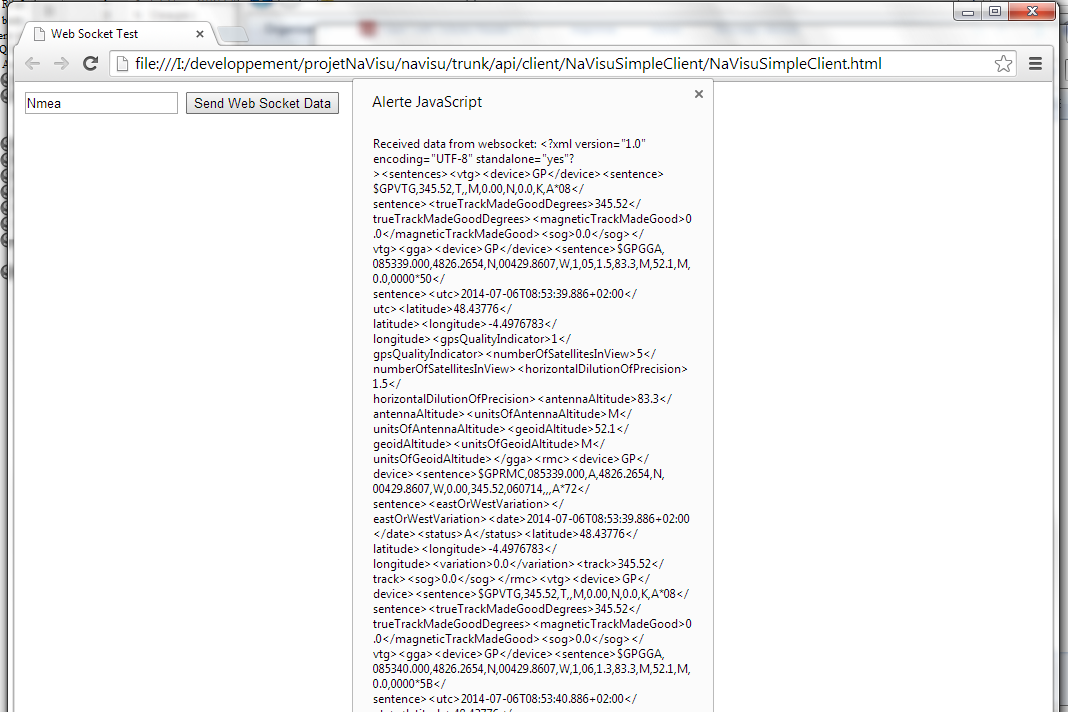
\includegraphics[width=16cm]{images/jsClient.png}
}
\begin{figure}[ht]
\caption{\label{0}\textit{Un client �l�mentaire en javascript}}
\end{figure}
\end{center}
%%%%%%%%%%%%%%%%%%%%%%%%%%%%%%%%%%%%%%%%%%%%%%%%%%%%%%%%%%%%%%%%%%%%%%%
%\chapter{Cr�ation d'un nouveau Display}

Ref : TV310315\_TU\_SM \hfill R�dacteur : Serge  Morvan \\


\section{Architecture}
\subsection{Principes}
Un {\tt Display} est un composant, au sens de C$^3$, il peut ainsi b�n�ficier des services du 
composant {\tt GuiAgent} par exemple. L'application n'a aucun lien cod� avec lui. Le design du nouveau compo\-sant 
est compl�tement s�par� du code.
Chaque �l�ment variable poss�de un id. Le contr�leur, instanci� par le {\tt Display} lors de l'initialisation
charge le fichier {\tt .fxml}. On retrouve dans le code du contr�leur les id de la partie graphique.
Pr�conisations : le composant graphique principal est un {\tt Group}, son id est : {\tt view}, chaque {\tt Display}
poss�de un bouton de fermeture, dont l'id est {\tt quit}. Le contr�leur h�rite de la classe {\tt Widget2D} qui offre 
les services de l'interactivit�.
 L'attribut {\tt KEY\_NAME}, ici : {\tt "InstrumentTemplate"} permet au Dock de le rechercher et de l'afficher, lorsque l'item
 associ� est s�lectionn�. Comme ci dessous dans la classe {\tt DockManagerImpl} du module {\tt navisu-app}, lors de
 la cr�ation du Dock :
 {\small 
\begin{verbatim}
instrumentsRadialMenu = RadialMenuBuilder.create()
.centralImage("instrumentsradialmenu150.png")
.createNode(0, "navigation.png",1,"ais.png",1,"template.png",(e)->open("InstrumentTemplate"))
.build();
\end{verbatim}
}
Le nouveau {\tt Display} devra s'enregistrer aupr�s du {\tt IntrumentDriverManagerServices}, dans la classe {\tt AppMain} du module {\tt navisu-launcher}.
{\small
\begin{verbatim}
 // deploy components
 LOGGER.info("\n"
 + componentManager.startApplication(DpAgentImpl.class,
 .....
  InstrumentTemplateImpl.class
  )
  );
  ......
  InstrumentTemplateServices instrumentTemplateServices 
                   = componentManager.getComponentService(InstrumentTemplateServices.class); 
  ......
  instrumentDriverManagerServices.registerNewDriver(instrumentTemplateServices.getDriver());
\end{verbatim}
}
\subsection{Diagramme UML}
La figure ci dessous pr�sente un diagramme simplifi� pour un {\tt Display} appel� {\tt InstrumentTemplate},
%%%%%%%%%%%%%%%%%%%%%%%%%%%%%%%%%%%%%%%%%%%%%%%%%%%%%%%%%%%%%%%%%%%%%%%
\begin{center}
	\framebox[1\width]{
		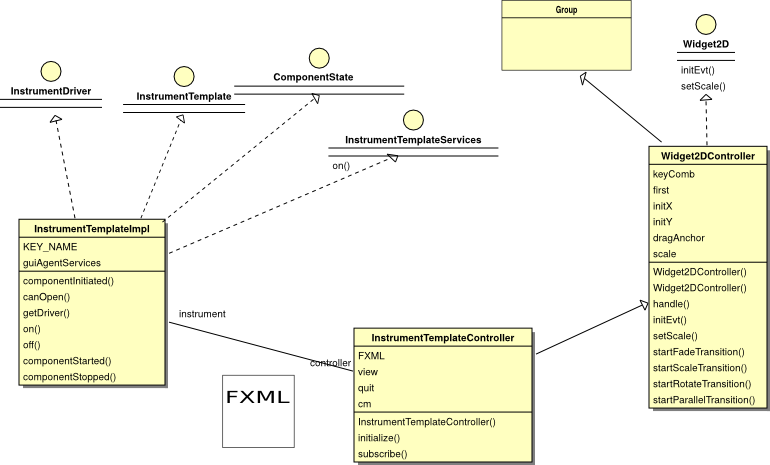
\includegraphics[width=16cm]{images/display/InstrumentTemplate.png}
	}
	\begin{figure}[ht]
		\caption{\label{0}\textit{Diagramme UML simplifi� d'un Display}}
	\end{figure}
\end{center}
%%%%%%%%%%%%%%%%%%%%%%%%%%%%%%%%%%%%%%%%%%%%%%%%%%%%%%%%%%%%%%%%%%%%%%%
\section{Cr�er un nouveau {\tt Display} : {\tt Compass}}
Reprendre le code du {\tt InstrumentTemplate}, �crire les interfaces {\tt Compass} et {\tt CompassServices}, impl�menter
les classes {\tt CompassImpl} et {\tt CompassControler}.Cr�er le fichier graphique {\tt compass.fxml}. Identifier par un id chaque variable.
Reprendre ces variables en mode public dans le contr�leur. Eventuellement ajouter des services, par d�faut
un {\tt Display} offre le service {\tt on()}. Impl�menter les contr�les.

%\chapter*{Cr�ation des menus}


\section{Objet}
Le but de cette section est d'expliquer la fa�on de rajouter un menu et ses sous-menus au Dock.
Un certain nombre de services doivent �tre activ�s, ou d�sactiv�s par l'utilisateur, pour cela, le menu
du Dock est privil�gi�. Le service � activer devra faire partie du groupe des {\tt Driver}: 
\hbox{}\vspace{0.2cm}

\begin{itemize}
 \item { \tt Driver } : pour l'ouverture de fichiers
 \item { \tt DDriver } : pour le parcours de r�pertoires   
 \item { \tt InstrumentDriver } : pour le choix d'un instrument   
 \item { \tt DatabaseDriver } : pour la connexion  � une base de donn�es
 \item { \tt WebDriver } : pour la connexion � un site web via un URL
 \item  \ldots autres � venir
\end{itemize}
Ce service doit �tre enregistr� dans le module {\tt navisu-launcher} :

\hbox{}\vspace{0.2cm}
{\small
\begin{boxedverbatim}
	
InstrumentDriverManagerServices instrumentDriverManagerServices =
         componentManager.getComponentService(InstrumentDriverManagerServices.class);
instrumentDriverManagerServices.init();
instrumentDriverManagerServices.registerNewDriver(sonarServices.getDriver());
instrumentDriverManagerServices.registerNewDriver(radarServices.getDriver());

\end{boxedverbatim}
}
\vspace{0.2cm}


Ensuite {\color{red}deux modules} sont concern�s, le module {\tt navisu-app} pour sp�cifier le nouvel item dans le Dock (ic�nes et code) et le module {\tt navisu-widgets} (ic�nes) car les {\tt RadialMenu} sont des widgets. Dans les deux cas les images sont plac�es dans les ressources, correspondant � l'arborescence des classes {\tt DockManagerImpl} et {\tt RadialMenu} respectivement. Dans la suite nous prendrons l'exemple de l'instanciation, du d�marrage ou de l'arr�t d'un {\tt Instrument}. Bien entendu cet {\tt Instrument} doit �tre impl�ment� au pr�alable.
\hbox{}\vspace{0.2cm}

{\small
	\begin{boxedverbatim}
		
public class SonarImpl
                  implements Sonar, SonarServices, InstrumentDriver, ComponentState {
	
\end{boxedverbatim}
}
\vspace{0.2cm}

\section{Le graphisme}
\subsection{Module \tt navisu-app}
	Dessiner l'ic�ne de l'item : � placer dans : \\
	{\tt bzh/terrevirtuelle/navisu/app/guiagent/impl/dock\_icons} des ressources
	%%%%%%%%%%%%%%%%%%%%%%%%%%%%%%%%%%%%%%%%%%%%%%%%%%%%%%%%%%%%%%%%%%%%%%%
	\begin{center}
		\framebox[1\width]{
			
\includegraphics[width=4cm]{images/instruments.png}
		}
		\begin{figure}[ht]
			\caption{\label{0}\textit{L'item Instruments}}
		\end{figure}
	\end{center}

	%%%%%%%%%%%%%%%%%%%%%%%%%%%%%%%%%%%%%%%%%%%%%%%%%%%%%%%%%%%%%%%%%%%%%%%
	\subsection{Module \tt navisu-widgets}
	%%%%%%%%%%%%%%%%%%%%%%%%%%%%%%%%%%%%%%%%%%%%%%%%%%%%%%%%%%%%%%%%%%%%%%%
	Dessiner les ic�nes de l'item central du {\tt RadialMenu} et de ses sous-items : � placer dans : \\
	{\tt bzh.terrevirtuelle.navisu.widgets.radialmenu.menu} des ressources.
	\begin{center}
		\framebox[1\width]{
			
\includegraphics[width=4cm]{images/instrumentsradialmenu.png}
		}
			\framebox[1\width]{
				
\includegraphics[width=2cm]{images/navigation.png}
			}
			\framebox[1\width]{
				
\includegraphics[width=2cm]{images/ais.png}
			}
			\framebox[1\width]{
				
\includegraphics[width=2cm]{images/aisradar.png}
			}
			\framebox[1\width]{
				
\includegraphics[width=2cm]{images/bathy.png}
			}
		\begin{figure}[ht]
			\caption{\label{0}\textit{L'ic�ne centrale de Instruments et les sous-items}}
		\end{figure}
	\end{center}
	%%%%%%%%%%%%%%%%%%%%%%%%%%%%%%%%%%%%%%%%%%%%%%%%%%%%%%%%%%%%%%%%%%%%%%%

\section{Le code}	
\subsection{Module \tt navisu-app}
 Dans la classe {\tt DockManagerImpl} du module {\tt navisu-app}, ajouter un item au Dock  :
\hbox{}\vspace{0.2cm}

{\small
	\begin{boxedverbatim}
		
public final DockItem[] ICONS = new DockItem[]{
	DockItemFactory.newImageItem("instruments", 
	     ICON_PATH + "dock_icons/instruments.png",
    	(e) -> {
        	instrumentsRadialMenu.setVisible(!instrumentsRadialMenu.isVisible());
    	}),
    	...
    	
\end{boxedverbatim}
}

\hbox{}\vspace{0.2cm}
		Ici {\tt "instruments"} correspond � l'infobulle associ�e, {\tt ICON\_PATH+"dock\_icons/instruments.png"} 
		est le chemin de l'image dans le r�pertoire {\tt resources}. Le dernier argument du constructeur est le
		callback associ�, g�n�ralement celui l�.
Appeler la m�thode de cr�ation du {\tt RadialMenu} associ� :

\hbox{}\vspace{0.2cm}
{\small
	\begin{boxedverbatim}
		
@Override
public void makeDock() {
    createDockWidget(scene);
    createBooksRadialWidget();
    createChartsRadialWidget();
		
    createInstrumentsRadialWidget();
	
    createMeteoRadialWidget();
    createTidesRadialWidget();
    createToolsRadialWidget();
    createNavigationRadialWidget();
}

\end{boxedverbatim}
}

\hbox{}\vspace{0.2cm}
Coder cette m�thode : le menu radial est cr�� � l'aide d'un {\tt RadialMenuBuilder}

\hbox{}\vspace{0.2cm}
{\small
	\begin{boxedverbatim}
		
	//--------------INSTRUMENTS------------------
private void createInstrumentsRadialWidget() {
    instrumentsRadialMenu = RadialMenuBuilder.create()
    .centralImage("instrumentsradialmenu.png")
    .createNode(0, "navigation.png", 0, "ais.png", 0, "aisradar.png", 
		                                                (e) -> open("AisRadar"))
    .createNode(0, "navigation.png", 1, "bathy.png", 0, "sonarOn.png",
		                                                (e) -> open("Sonar"))
    .build();
		
    instrumentsRadialMenu.setLayoutX((width / 2) - 40);
    instrumentsRadialMenu.setLayoutY(height / 2);
    root.getChildren().add(instrumentsRadialMenu);
	
    radialMenus.add(instrumentsRadialMenu);
	}
	
\end{boxedverbatim}
}

\hbox{}\vspace{0.2cm}
\begin{itemize}
	\item La m�thode {\tt createNode} va pr�ciser pour chaque item, son placement, ses images associ�es et son callback.
	\begin{itemize}
		\item Un choix d'ergonomie a �t� fait, les menus radiaux ont deux couches de sous-menus puis des feuilles, les feuilles correspondent aux actions.
		\item Dans la premi�re couche les segments sont num�rot�s : 0, 1, 2, ... Dans l'exemple un seul segment,
		son ic�ne est {\tt navigation.png"}
		\item Dans la deuxi�me couche, idem, les segments sont num�rot�s : 0, 1, 2, ...Dans l'exemple deux
		segments, les ic�nes {\tt ais.png} et {\tt bathy.png}
		\item Chaque segment re�oit les feuilles correspondant aux items, ici un item par segment. 
		les images {\tt aisradar.png} et {\tt sonarOn.png} respectivement.
		\item Enfin, le dernier argument correspond au callback associ� � cet item.
	\end{itemize}
\end{itemize}

	%%%%%%%%%%%%%%%%%%%%%%%%%%%%%%%%%%%%%%%%%%%%%%%%%%%%%%%%%%%%%%%%%%%%%%%
	\begin{center}
		\framebox[1\width]{
			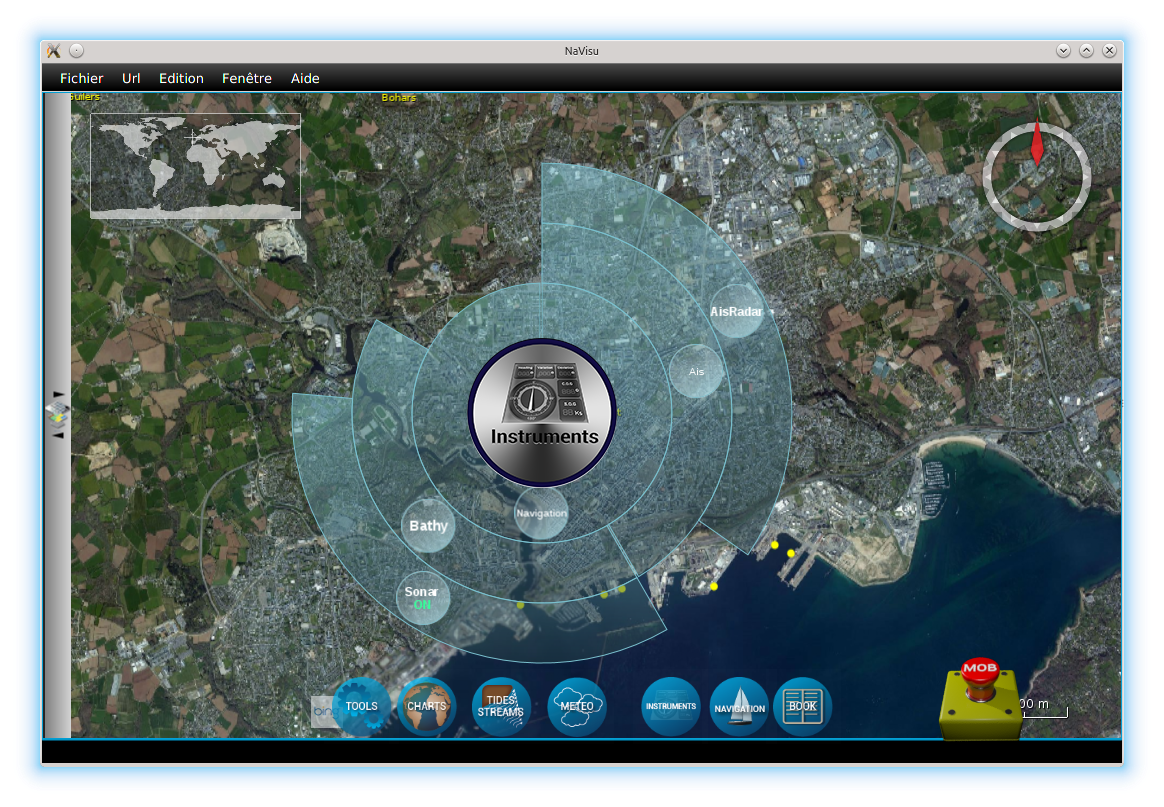
\includegraphics[width=16cm]{images/menu.png}
		}
		\begin{figure}[ht]
			\caption{\label{0}\textit{Le menu Instruments}}
		\end{figure}
	\end{center}
	
	%%%%%%%%%%%%%%%%%%%%%%%%%%%%%%%%%%%%%%%%%%%%%%%%%%%%%%%%%%%%%%%%%%%%%%%	
 	\subsection{Choix des {\tt callbacks}}	
 	La plupart du temps les callbacks associ�s aux items n'ont pas besoin d'�tre cod�s, il sont fournis par \nav
 	. Ci apr�s la liste non exhaustive des calbacks et des cas d'utilisation.
 	\begin{itemize}
\item Cas d'un instrument : l'argument correspond au nom de l'instrument � activer.

	\hbox{}\vspace{0.2cm}
	{\small
		\begin{boxedverbatim}
		
private void open(String keyName) {
    instrumentDriverManagerServices.open(keyName);
    clear();
}

\end{boxedverbatim}
}

\newpage 
\item Cas d'ouverture d'un fichier : le premier argument est le {\tt KEY\_NAME} du {\tt Driver} sachant interpr�ter ces fichiers : Sedimentology, Currents, \ldots Le deuxi�me argument le ou les extensions des fichiers : {\tt .shp, .SHP} ou {\tt .000} par exemple.

\hbox{}\vspace{0.2cm}
	{\small
		\begin{boxedverbatim}
			
private void open(String description, String... des) {
    String[] tab = new String[des.length];	
    int i = 0;
    for (String s : des) {
        tab[i] = "*" + s;
        i++;
    }
    driverManagerServices.open(description, tab);
    clear();
}

\end{boxedverbatim}
}

\hbox{}\vspace{0.2cm}
\item Connexion � une base de donn�es :

\hbox{}\vspace{0.2cm}
{\small
	\begin{boxedverbatim}
		
private void openDB(String dbName, String hostName, String protocol, String port,
String driverName, String userName, String passwd) {
    databaseDriverManagerServices.connect(dbName, hostName, protocol, 
                                            port, driverName, userName, passwd);
    clear();
}
		
	\end{boxedverbatim}
}

	\hbox{}\vspace{0.2cm}
\nav\ g�re autant de bases de donn�es qu'il est n�cessaire, elles doivent �tre install�es au pr�alable, sauf pour une base embarqu�e. C'est l'API JDBC qui est exhib�e comme un ensemble de services.

\end{itemize}
\hbox{}\vspace{0.2cm}

	\subsection{Module  \tt navisu-widgets}
	Pas de code � �crire, il faut simplement placer les images correspondant au menu et � ses items, dans le fichier {\tt resources}.
%%%%%%%%%%%%%%%%%%%%%%%%%%%%%%%%%%%%%%%%%%%%%%%%%%%%%%%%%%%%%%%%%%%%%%%
\section{Principe des {\tt DriverManager}}
Comme il a �t� dit dans la pr�face, les services accessibles � partir du menu doivent s'enregistrer, voici l'explication. Le premier principe respect� est {\color{red} l'inversion de d�pendance} : la logique de l'application, contenue dans le module {\tt navisu-app} ne doit pas d�pendre des modules quelle active :
%%%%%%%%%%%%%%%%%%%%%%%%%%%%%%%%%%%%%%%%%%%%%%%%%%%%%%%%%%%%%%%%%%%%%%%
\begin{center}
	\framebox[1\width]{
		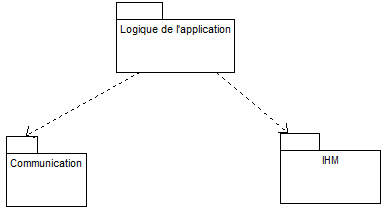
\includegraphics[width=9cm]{images/dip_0.png}
	}
	\begin{figure}[ht]
		\caption{\label{0}\textit{Une modification de l'IHM va impacter l'application}}
	\end{figure}
\end{center}
%%%%%%%%%%%%%%%%%%%%%%%%%%%%%%%%%%%%%%%%%%%%%%%%%%%%%%%%%%%%%%%%%%%%%%%	
La logique de l'application  doit s'appuyer sur des services :
%%%%%%%%%%%%%%%%%%%%%%%%%%%%%%%%%%%%%%%%%%%%%%%%%%%%%%%%%%%%%%%%%%%%%%%
\begin{center}
	\framebox[1\width]{
		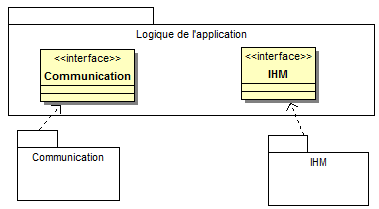
\includegraphics[width=9cm]{images/dip_1.png}
	}
	\begin{figure}[ht]
		\caption{\label{0}\textit{Si les contrats de services sont respect�s, un changement du code de l'IHM ne concerne pas l'application}}
	\end{figure}
\end{center}
%%%%%%%%%%%%%%%%%%%%%%%%%%%%%%%%%%%%%%%%%%%%%%%%%%%%%%%%%%%%%%%%%%%%%%%	
Le deuxi�me principe est celui de  {\color{red}pas de d�pendances cycliques} :
%%%%%%%%%%%%%%%%%%%%%%%%%%%%%%%%%%%%%%%%%%%%%%%%%%%%%%%%%%%%%%%%%%%%%%%
\begin{center}
	\framebox[1\width]{
		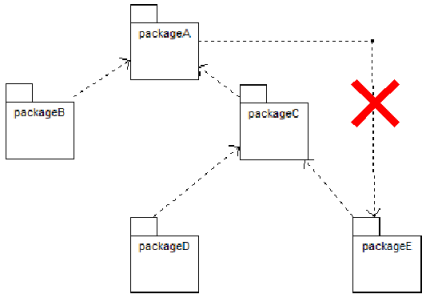
\includegraphics[width=9cm]{images/adp_1.png}
	}
	\begin{figure}[ht]
		\caption{\label{0}\textit{Gradle d�tectera un tel probl�me}}
	\end{figure}
\end{center}
%%%%%%%%%%%%%%%%%%%%%%%%%%%%%%%%%%%%%%%%%%%%%%%%%%%%%%%%%%%%%%%%%%%%%%%	

Dans chaque fichier {\tt build.gradle} on trouve les d�pendances du  module, par exemple dans le sous-projet {\tt navisu-intruments}  

\hbox{}\vspace{0.2cm}
{\small
	\begin{boxedverbatim}
		
dependencies {
    compile project(':navisu-core')
    compile project(':navisu-client')
    compile project(':navisu-domain')
    compile project(':navisu-app')
    compile project(':navisu-bathymetry')
    compile fileTree(dir: 'lib', include: '*.jar')
}

	\end{boxedverbatim}
}
\hbox{}\vspace{0.2cm}

Si le module {\tt navisu-app} devait instancier un {\tt Intrument} directement, il devrait connaitre, donc d�pendre du module {\tt navisu-intruments} ce qui constitue une rupture du principe num�ro deux.
Au lieu de cela les diff�rents {\tt Driver} s'inscrivent aupr�s de leur {\tt DriverManager} sp�cifique, 
ensuite lors d'une requ�te lanc�e par les callbacks du dock, le {\tt Driver} r�pondant aux crit�res de s�lection est activ�.

\hbox{}\vspace{0.2cm}
{\small
	\begin{boxedverbatim}
		
// class InstrumentDriverManagerImpl
	
protected List<InstrumentDriver> availableDriverList = new ArrayList<>();
	
@Override
public void registerNewDriver(InstrumentDriver driver) {
    Checker.notNull(driver, "Driver must not be null.");
    this.availableDriverList.add(driver);
}

@Override
public void open(String category) {
    InstrumentDriver driver = findDriver(category);
    if (driver != null) {
        driver.on();
    }else{
        System.out.println("Unrecognized instrument");
    }
}

protected InstrumentDriver findDriver(String category) {
    InstrumentDriver compatibleDriver = null;
    for (InstrumentDriver driver : this.availableDriverList) {
        if (driver.canOpen(category)) {
            compatibleDriver = driver;
            break;
        }
    }
    return compatibleDriver;
}
					
	\end{boxedverbatim}
}

\newpage
Exemple pour la classe {\tt Sonar} les m�thodes r�pondant au {\tt DriverManager}

\hbox{}\vspace{0.2cm}
{\small
	\begin{boxedverbatim}
		
// public class SonarImpl
              implements Sonar, SonarServices, InstrumentDriver, ComponentState {
              	
 private final String NAME = "Sonar";
 		
@Override
public boolean canOpen(String category) {
    return category.equals(NAME);
}
@Override
    public void on() {
        ...
}					
\end{boxedverbatim}
}
%\chapter{Gestion des �v�nements}


\section{Architecture}
\subsection{Principes}
1- Pour les objets en overlay, c'est du JavFX 

1.1 charg� depuis un fichier FXML :

quit.setOnMouseClicked((MouseEvent event) -> {
	instrument.off();
});

quit est ici un Button.

1.2 H�ritant de Widget2DController, par exemple :

public class RouteEditorController
extends Widget2DController

Il y a d�j� un comportement par d�faut, apparition, disparition, d�placement, ... Voir le d�tail dans la classe Widget2DController, losr de l'instanciation on peut personnaliser le widget : 

routeEditorController = new RouteEditorController(this,
layersManagerServices ,
KeyCode.M, KeyCombination.CONTROL\_DOWN);
La touche M, permettra de faire disparaitre ce widget.

2- Pour les objets venant de WorldWind, c'est du Swing, il suffit de mettre l'objet WorldWindow � l'�coute d'un �v�nement de s�lection par exemple et de filtrer cet evt : 

2.1 Globalement :
\begin{verbatim}
private void addListeners() {
	wwd.addSelectListener((SelectEvent event) -> {
		Object o = event.getTopObject();
		if (event.isLeftClick() && o != null) {
			if (o.getClass() == PointPlacemark.class) {
				System.out.println("OK");
			}
		}
	});
}
\end{verbatim}
On voit ici que tous les objets de type PointPlacemark, au moins pour les couches sensibles aux �v�nements, seront s�lectionn�s.
Pour r�agir � cet evt, cel� peut convenir pour afficher leur nom par exemple, mais pour pour une action sp�cifique, c'est sans doute trop g�n�ral. Il faut donc filtrer des objets dont la vue est un PointPlacemark, mais qui ont un type particulier.

Une solution : cr�er la classe Poimark : 
\begin{verbatim}
public class Poimark extends PointPlacemark{
	
	public Poimark(Position pstn) {
		super(pstn);
	}
}
\end{verbatim}
Ensuite filtrer les Poimark : 
\begin{verbatim}
private void addListeners() {
	wwd.addSelectListener((SelectEvent event) -> {
		Object o = event.getTopObject();
		if (event.isLeftClick() && o != null) {
			if (o.getClass() == Poimark.class) {
				System.out.println("Action");
			}
		}
	});
}
\end{verbatim}
Enfin instancier des Poimark plut�t que de simples PointPlacemark :

\begin{verbatim}
public Set<Pair<Double, Double>> showPoi(Map<Pair<Double, Double>, String> data) {
	Set<Pair<Double, Double>> latLonSet = data.keySet();
	
	latLonSet.stream().map((ll) -> {
		String imageAddress = NavigationIcons.ICONS.get(ICON_NAME);
		
		Poimark poimark = new Poimark(Position.fromDegrees(ll.getX(), ll.getY(), 0));
		poimark.setAltitudeMode(WorldWind.CLAMP_TO_GROUND);
		poimark.setValue(AVKey.DISPLAY_NAME, data.get(ll));
		PointPlacemarkAttributes normalAttributes = new PointPlacemarkAttributes();
		normalAttributes.setImageAddress(imageAddress);
		normalAttributes.setScale(0.4);
		poimark.setAttributes(normalAttributes);
		return poimark;
	}).forEach((placemark) -> {
	sailingDirectionsIconsLayer.addRenderable(placemark);
});

return latLonSet;
}
\end{verbatim}
%%%%%%%%%%%%%%%%%%%%%%%%%%%%%%%%%%%%%%%%%%%%%%%%%%%%%%%%%%%%%%%%%%%%%%%%
\chapter{Cartographie}
\section{Pr�sentation}

\nav\ utilise les cartes raster BSB/KAP. Avant d'utiliser vos cartes il est
n�cessaire d'op�rer un pr�-traitement, c'est l'op�ration de tuilage : la carte
au format KAP, de 1 � plusieurs Mo, sera transform�e en plusieurs sous images
ou tuiles. Les r�pertoires o� sont plac�s les cartes et les tuiles doivent �tre
renseign�s dans l'application.
\subsection{La projection Equirectangulaire}
%%%%%%%%%%%%%%%%%%%%%%%%%%%%%%%%%%%%%%%%%%%%%%%%%%%%%%%%%%%%%%%%%%%%%%
\nav, s'appuyant sur
\href{http://goworldwind.org/}{WorldWind},
utilise une projection cylindrique simple (appel�e projection
Equirectangulaire ou Plate Carr�e) avec comme r�f�rentiel g�od�sique le WGS84. Dans la projection Equirectangulaire
  l'instersection avec les m�ridiens se fait � angle droit, 
  mais contrairement � la projection Mercator, les parall�les sont des lignes
  droites �quidistantes.
%%%%%%%%%%%%%%%%%%%%%%%%%%%%%%%%%%%%%%%%%%%%%%%%%%%%%%%%%%%%%%%%%%%%%%%
\begin{center}
\framebox[1\width]{
	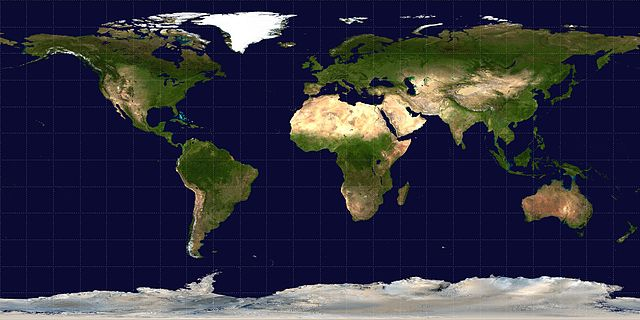
\includegraphics[width=16cm]{images/carto/Equirectangular-projection.png}
}
\begin{figure}[ht]
\caption{\label{equiProj}\textit{Projection �quirectangulaire}}
\end{figure}
\end{center}
%%%%%%%%%%%%%%%%%%%%%%%%%%%%%%%%%%%%%%%%%%%%%%%%%%%%%%%%%%%%%%%%%%%%%%%
Pour plus
d'informations sur le sujet consulter, par exemple,  le site du
``Intergovernmental Committee on Surveying and Mapping ``(ICSM) :
%%%%%%%%%%%%%%%%%%%%%%%%%%%%%%%%%%%%%%%%%%%%%%%%%%%%%%%%%%%%%%%%%%%%%%%

{
	\tt
	 \href{http://www.icsm.gov.au/mapping/about\_projections.html}{http://www.icsm.gov.au/mapping/about\_projections.html}
}\\

\vspace{.2cm}
%%%%%%%%%%%%%%%%%%%%%%%%%%%%%%%%%%%%%%%%%%%%%%%%%%%%%%%%%%%%%%%%%%%%%%%
Et pour un expos� plus large des probl�mes de projection :\\

\vspace{.2cm}
%%%%%%%%%%%%%%%%%%%%%%%%%%%%%%%%%%%%%%%%%%%%%%%%%%%%%%%%%%%%%%%%%%%%%%%
{
\tt 
	 \href{http://kartoweb.itc.nl/geometrics/}{http://kartoweb.itc.nl/geometrics/}
}
%%%%%%%%%%%%%%%%%%%%%%%%%%%%%%%%%%%%%%%%%%%%%%%%%%%%%%%%%%%%%%%%%%%%%%%

\subsection{Tuilage}
\subsubsection{Le principe}
Comme la plupart des applications g�or�f�renc�es (GoogleEarth, Yahoo, Bing,
\ldots) pour fournir un niveau de d�tail important et une bonne fluidit�,
\nav\ utilise la m�thode du tuilage des cartes. Les images affich�es sont de
256x256 pixels. Elles sont choisies suivant le niveau de zoom et l'emplacement
g�ographique, l'affichage � l'�cran est recr�� dynamiquement.
Chaque carte est constitu�e d'un r�pertoire, puis de nombreux sous-r�pertoires
num�rot�s comme suit :
%%%%%%%%%%%%%%%%%%%%%%%%%%%%%%%%%%%%%%%%%%%%%%%%%%%%%%%%%%%%%%%%%%%%%%%
\begin{center}
\framebox[1\width]{
	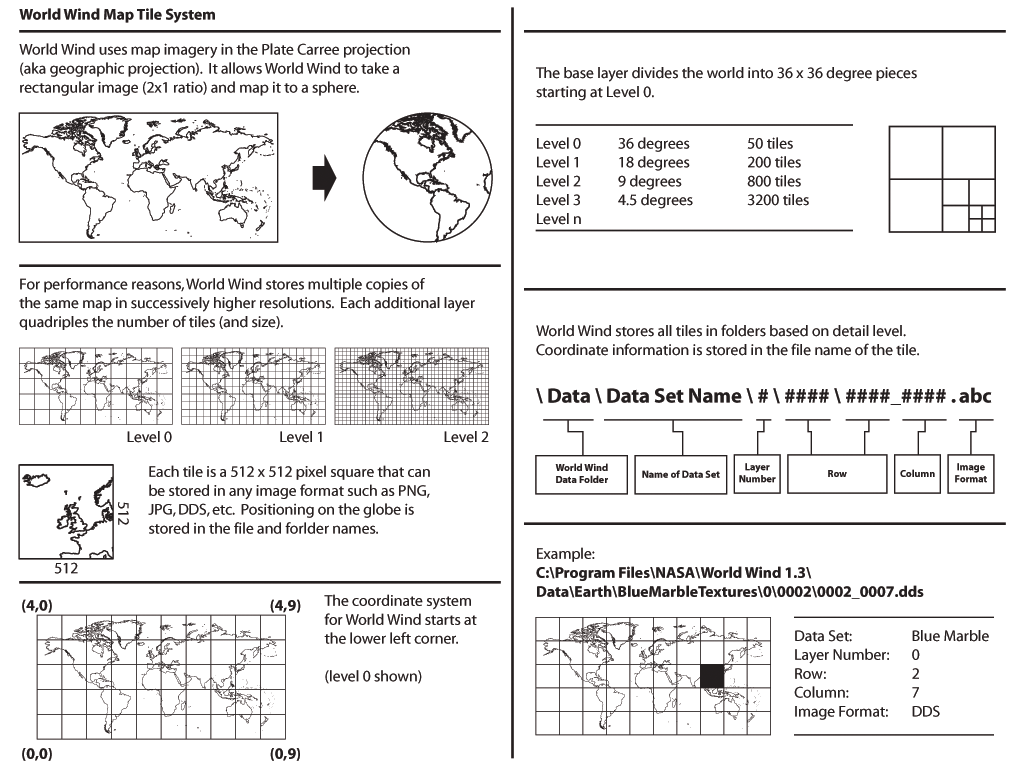
\includegraphics[width=16cm]{images/carto/Worldwind_tile_system.png}
}
\begin{figure}[ht]
\caption{\label{wwTiles}\textit{Conventions de la num�rotation des
tuiles WorldWind}}
\end{figure}
\end{center}
 Lors d'un
premier acc�s ces images peuvent provenir de diff�rents sites internet, elles
sont mises en cache sur le disque utilisateur. Lors des acc�s suivants
l'application commence par chercher dans le cache. Elles peuvent �tre d�s le
d�part �tre mise dans le cache.\\
 Sous Windows 7 par d�faut WorldWind utilise le
r�pertoire :
\begin{verbatim} C:\ProgramData\WorldWindData \end{verbatim} 

Pour plus de d�tails sur le tuilage, voir :

%%%%%%%%%%%%%%%%%%%%%%%%%%%%%%%%%%%%%%%%%%%%%%%%%%%%%%%%%%%%%%%%%%%%%%%
\begin{center}
	 \href{http://www.worldwindcentral.com/wiki/Tiling\_System}{http://www.worldwindcentral.com/wiki/Tiling\_System}
\end{center}
%%%%%%%%%%%%%%%%%%%%%%%%%%%%%%%%%%%%%%%%%%%%%%%%%%%%%%%%%%%%%%%%%%%%%%%
\section{Cartographie raster}
\subsection{Les cartes BSB/KAP}
 L'utilisateur peut d�finir son
propre r�pertoire pour passer facilement d'un ordinateur � un autre, sans avoir � recopier les donn�es.


%%%%%%%%%%%%%%%%%%%%%%%%%%%%%%%%%%%%%%%%%%%%%%%%%%%%%%%%%%%%%%%%%%%%%%%
\begin{center}
\framebox[1\width]{
	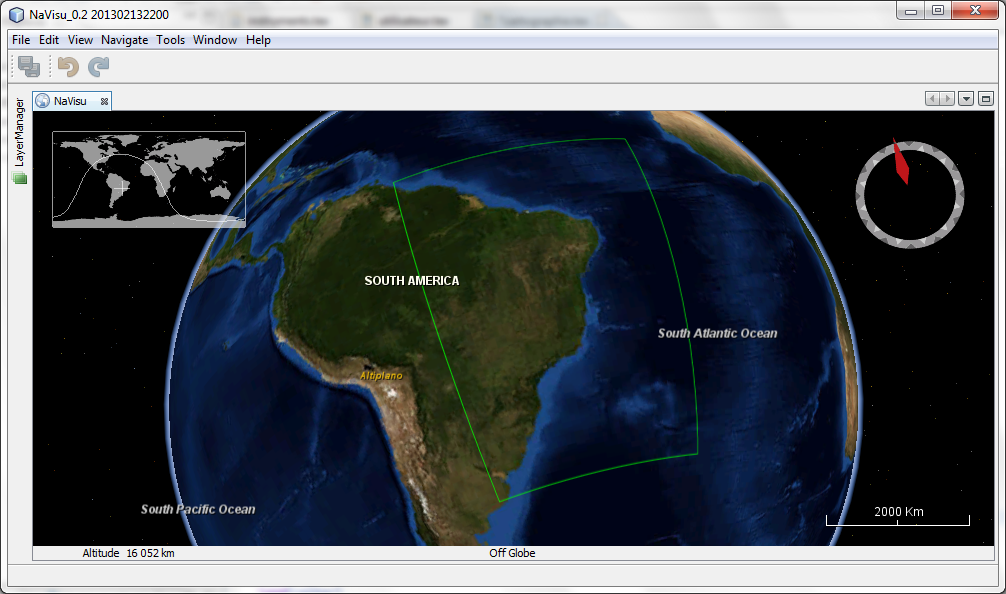
\includegraphics[width=16cm]{images/carto/0.png}
}
\begin{figure}[ht]
\caption{\label{carte0}\textit{Fronti�res d'une carte}}
\end{figure}
\end{center}
%%%%%%%%%%%%%%%%%%%%%%%%%%%%%%%%%%%%%%%%%%%%%%%%%%%%%%%%%%%%%%%%%%%%%%%
Les fronti�res sont en vert : la carte 101.KAP est dans le r�pertoire d�sign� et
la carte a �t� tuil�e, les tuiles sont dans le cache d�sign�. Si les tuiles ne
sont pas dans le cache les polygones fronti�re sont rouges.
%%%%%%%%%%%%%%%%%%%%%%%%%%%%%%%%%%%%%%%%%%%%%%%%%%%%%%%%%%%%%%%%%%%%%%%
\begin{center}
\framebox[1\width]{
	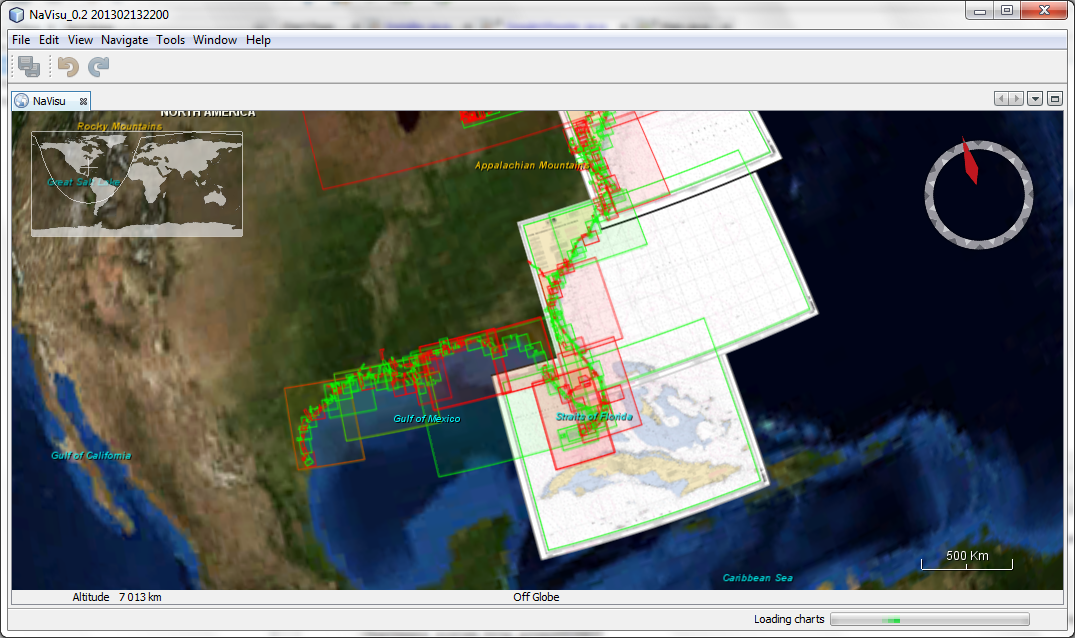
\includegraphics[width=16cm]{images/carto/3.png}
}
\begin{figure}[ht]
\caption{\label{usa}\textit{Les Etats Unis}}
\end{figure}
\end{center}
%%%%%%%%%%%%%%%%%%%%%%%%%%%%%%%%%%%%%%%%%%%%%%%%%%%%%%%%%%%%%%%%%%%%%%%
%%%%%%%%%%%%%%%%%%%%%%%%%%%%%%%%%%%%%%%%%%%%%%%%%%%%%%%%%%%%%%%%%%%%%%%
\begin{center}
\framebox[1\width]{
	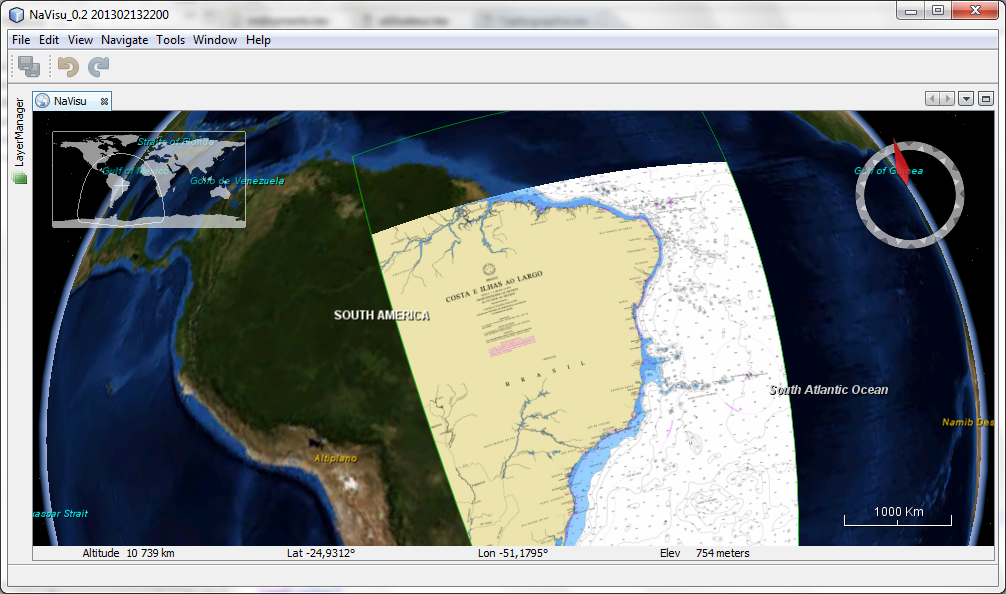
\includegraphics[width=16cm]{images/carto/1.png}
}
\begin{figure}[ht]
\caption{\label{carte1}\textit{Affichage de la carte}}
\end{figure}
\end{center}
%%%%%%%%%%%%%%%%%%%%%%%%%%%%%%%%%%%%%%%%%%%%%%%%%%%%%%%%%%%%%%%%%%%%%%%
Double clic � l'int�rieur du polygone : affichage de la carte, d�s que
l'altitude le permet.
Ici la distance fait que les tuiles les plus hautes en latitude ne s'affichent pas encore.
%%%%%%%%%%%%%%%%%%%%%%%%%%%%%%%%%%%%%%%%%%%%%%%%%%%%%%%%%%%%%%%%%%%%%%%
\begin{center}
\framebox[1\width]{
	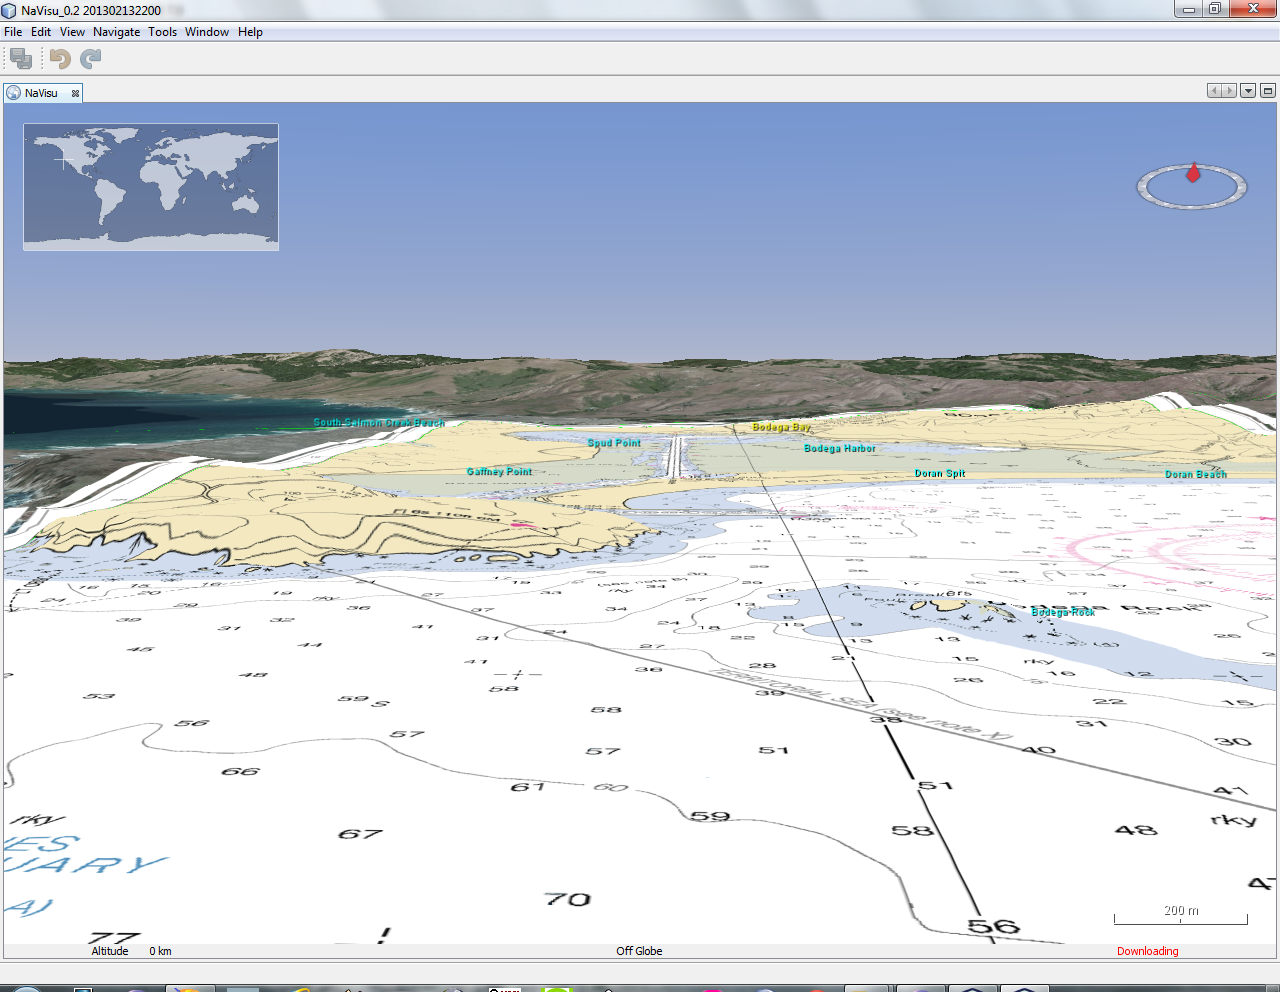
\includegraphics[width=16cm]{images/carto/2.png}
}
\begin{figure}[ht]
\caption{\label{details}\textit{Niveaux de d�tail et la 3D}}
\end{figure}
\end{center}
%%%%%%%%%%%%%%%%%%%%%%%%%%%%%%%%%%%%%%%%%%%%%%%%%%%%%%%%%%%%%%%%%%%%%%%
\subsection{Acquisition}
Quelques sites pour obtenir des cartes raster au format BSB/KAP : 
%%%%%%%%%%%%%%%%%%%%%%%%%%%%%%%%%%%%%%%%%%%%%%%%%%%%%%%%%%%%%%%%%%%%%%%

{
\tt\small
	 \href{http://marine.geogarage.com/}{http://marine.geogarage.com/}
	 
	 \vspace{.2cm}
	\href{http://www.justmagic.com/RasterChart2BSB.html}{http://www.justmagic.com/RasterChart2BSB.html}
	
	\vspace{.2cm}
	 \href{https://www.mar.mil.br/dhn/chm/cartas/download/cartasbsb/cartas\_eletronicas\_Internet.htm}{https://www.mar.mil.br/dhn/chm/cartas/download/cartasbsb/cartas\_eletronicas\_Internet.htm}
	
	\vspace{.2cm}
	 \href{http://www.nauticalcharts.noaa.gov/mcd/Raster/index.htm}{http://www.nauticalcharts.noaa.gov/mcd/Raster/index.htm}
	
	 \vspace{.2cm}
	 \href{http://www.1yachtua.com/}{http://www.1yachtua.com/}
	 
}
%%%%%%%%%%%%%%%%%%%%%%%%%%%%%%%%%%%%%%%%%%%%%%%%%%%%%%%%%%%%%%%%%%%%%%%


%%%%%%%%%%%%%%%%%%%%%%%%%%%%%%%%%%%%%%%%%%%%%%%%%%%%%%%%%%%%%%%%%%%%%%%%
\chapter*{Module STL}
\section{Pr�sentation}
Le module {\tt navisu-stl} permet la cr�ation d'objets g�or�f�renc�s � l'aide d'imprimantes 3D. Ces objets sont des mod�les num�riques de terrain (MNT), des donn�es cartographiques (S57 de l'IHO) ou des donn�es bathym�triques.
Le process : apr�s s�lection, les donn�es au format interne NaVisu sont transform�es au format {\tt x3D}.
Ces fichiers sont import�s dans le logiciel Blender, pour la g�n�ration de simples facettes triangulaires pour l'ensemble des donn�es, car le fichier d'origine contient des primitives {\tt x3D} non lues par les logiciels d'impression 3D. Ces m�mes fichiers sont ensuite r�export�s au format {\tt x3D}. Ils sont alors import�s dans le logiciel  
\href{https://ultimaker.com/en/products/cura-software}{Cura}, il permet le contr�le et la simulation des diff�rentes couches d'impression, puis exporte les donn�es au format STL et au format de la machine cible pour impression. 

%%%%%%%%%%%%%%%%%%%%%%%%%%%%%%%%%%%%%%%%%%%%%%%%%%%%%%%%%%%%%%%%%%%%%%%
\begin{center}
	\framebox[1\width]{
		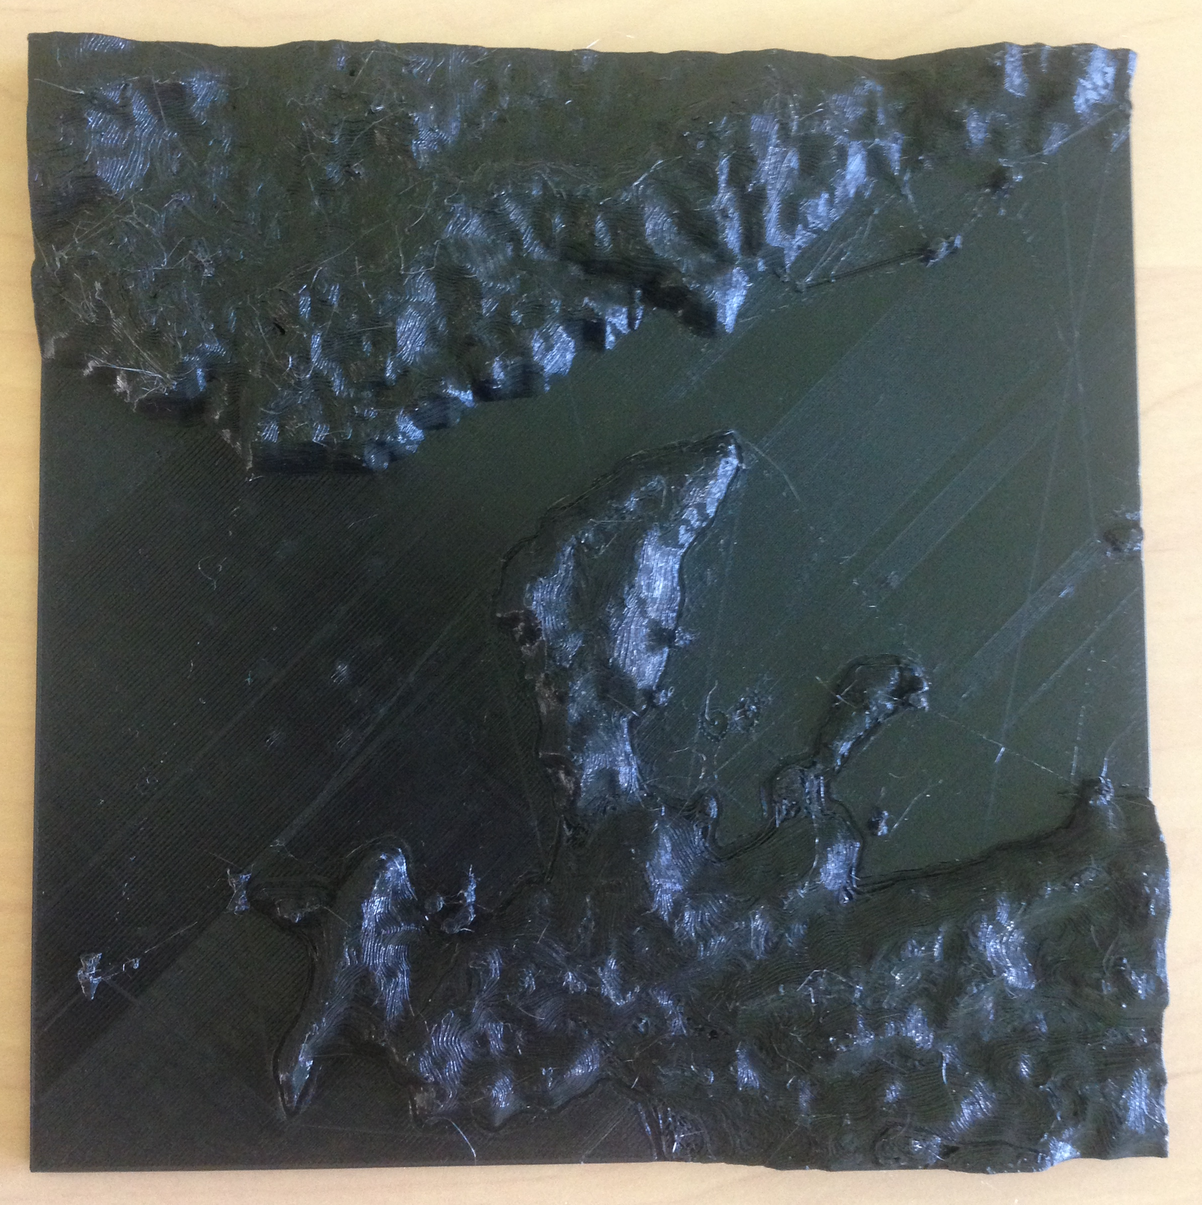
\includegraphics[width=10cm]{images/stl/gouletBrest.png}
	}
	\begin{figure}[ht]
		\caption{\label{sdModel}\textit{Premier prototype d'impression 3D, brut de fabrication : Le goulet de Brest}}
	\end{figure}
\end{center}
%%%%%%%%%%%%%%%%%%%%%%%%%%%%%%%%%%%%%%%%%%%%%%%%%%%%%%%%%%%%%%%%%%%%%%%
\section{Cartographie et MNT}
\subsection{S�lection des zones � imprimer}
A partir du catalogue de cartes, s�lectionner une carte : {\tt\bf F1 + Clic droit} sur l'emprise de la carte. Puis � l'aide l'ihm, pr�ciser les tuiles � g�n�rer. Pour le moment, les tuiles, sont carr�es comme les plateaux des imprimantes.
%%%%%%%%%%%%%%%%%%%%%%%%%%%%%%%%%%%%%%%%%%%%%%%%%%%%%%%%%%%%%%%%%%%%%%%
\begin{center}
	\framebox[1\width]{
		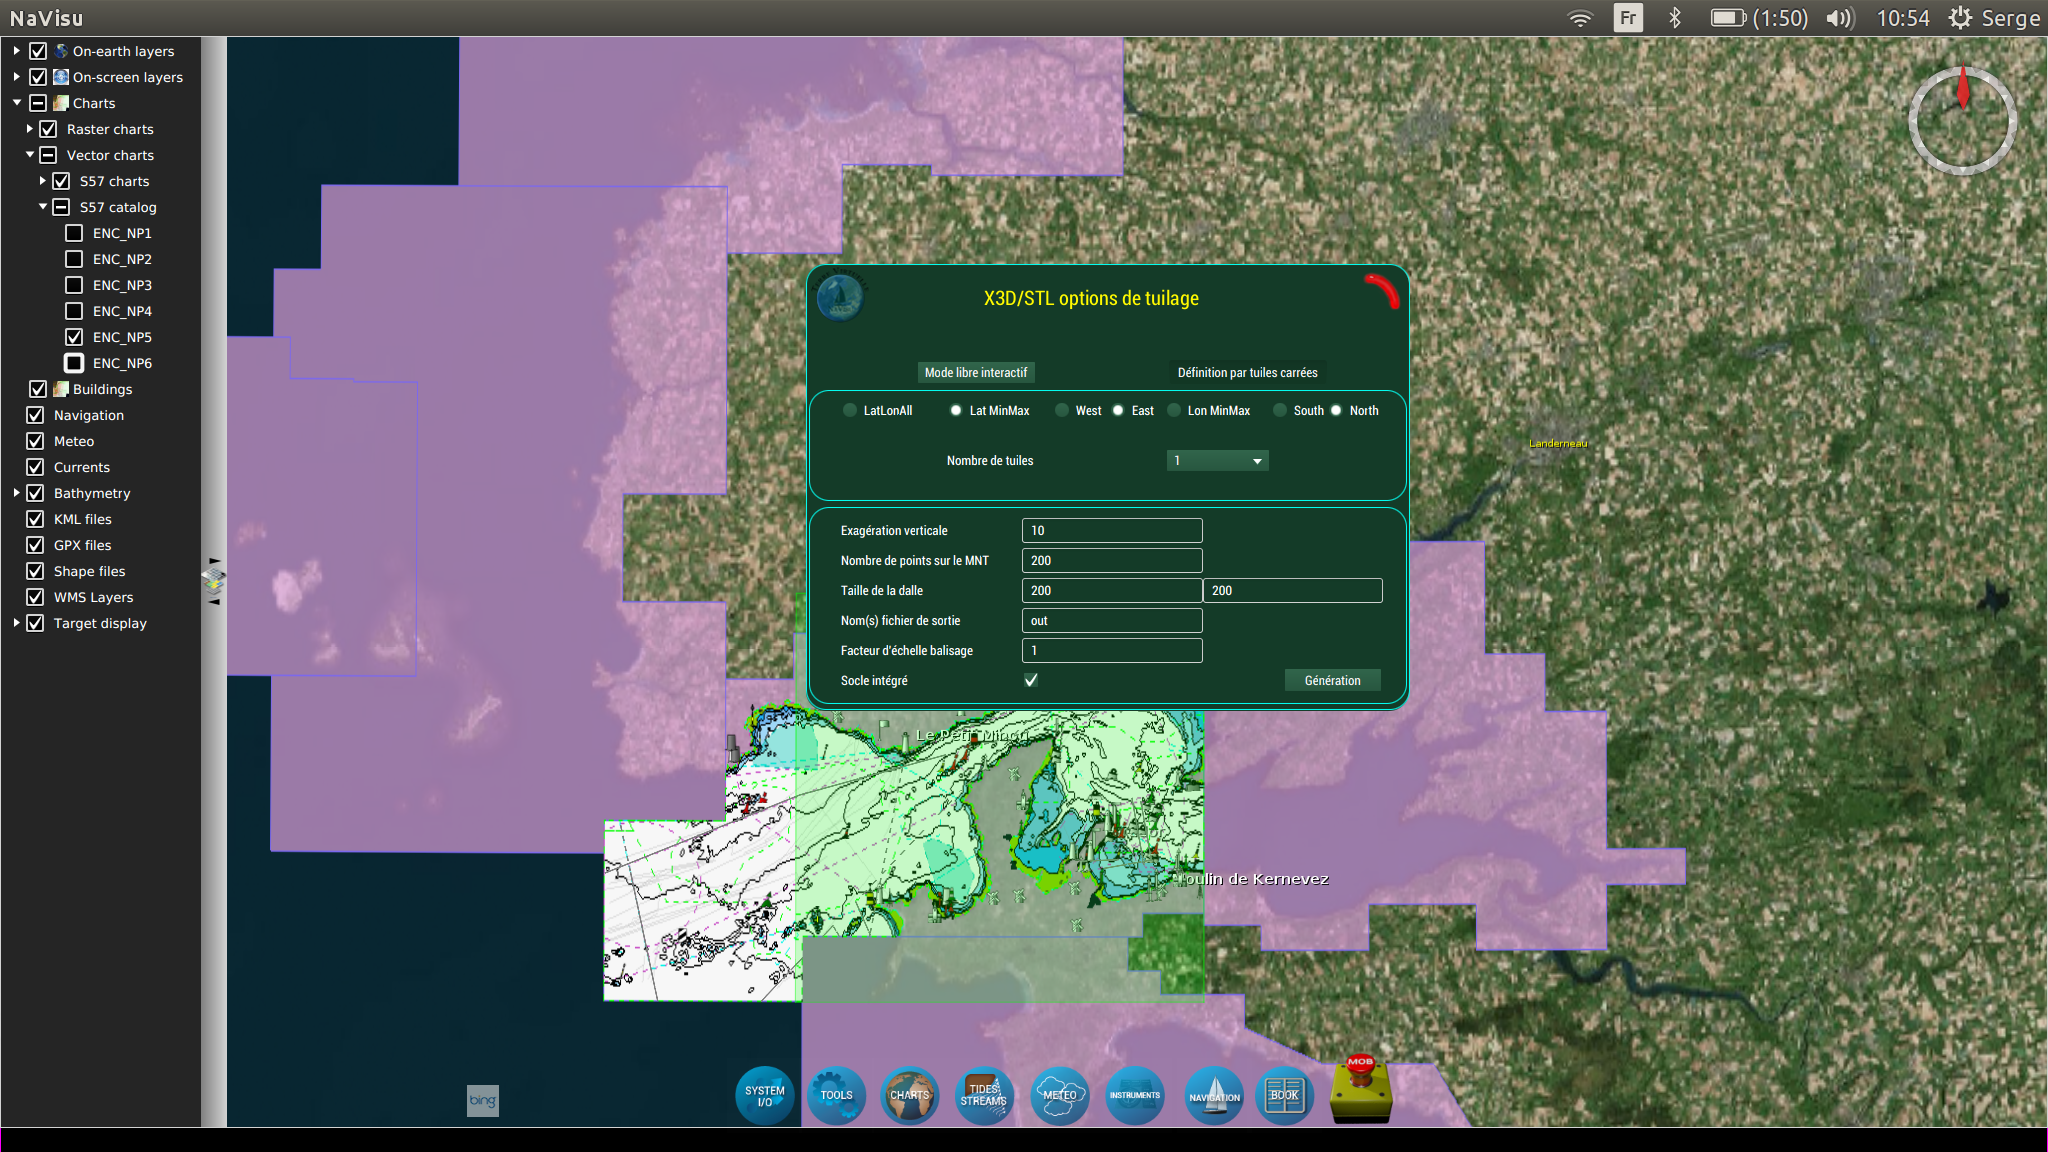
\includegraphics[width=15cm]{images/stl/choixTuiles.png}
	}
	\begin{figure}[ht]
		\caption{\label{sdModel}\textit{Choix de la zone � imprimer � partir du catalogue de cartes S57.}}
	\end{figure}
\end{center}
%%%%%%%%%%%%%%%%%%%%%%%%%%%%%%%%%%%%%%%%%%%%%%%%%%%%%%%%%%%%%%%%%%%%%%%

%%%%%%%%%%%%%%%%%%%%%%%%%%%%%%%%%%%%%%%%%%%%%%%%%%%%%%%%%%%%%%%%%%%%%%%
\begin{center}
	\framebox[1\width]{
		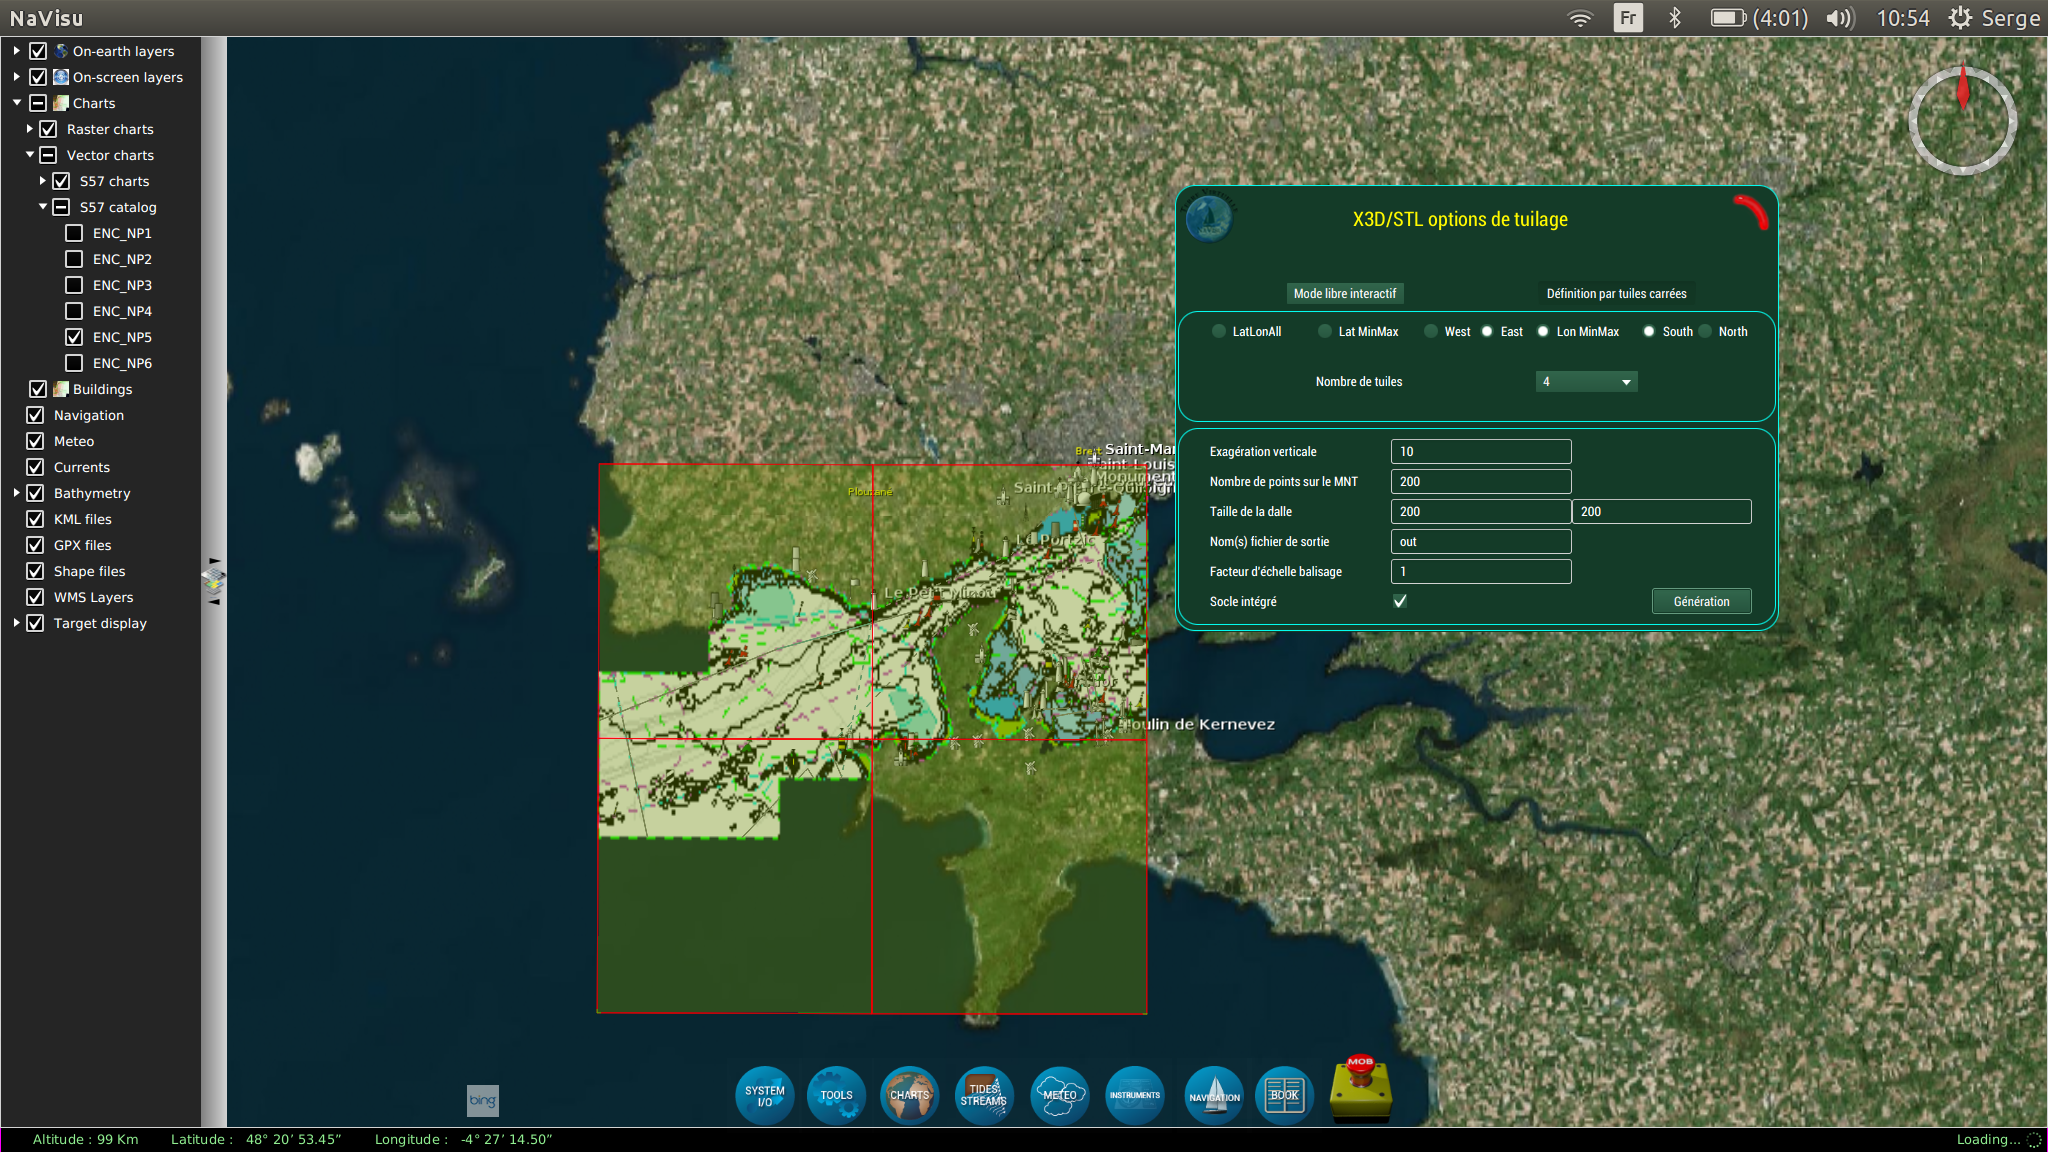
\includegraphics[width=15cm]{images/stl/generationTuiles.png}
	}
	\begin{figure}[ht]
		\caption{\label{sdModel}\textit{S�lection des tuiles, position, nombre et g�n�ration du fichier x3D.}}
	\end{figure}
\end{center}
%%%%%%%%%%%%%%%%%%%%%%%%%%%%%%%%%%%%%%%%%%%%%%%%%%%%%%%%%%%%%%%%%%%%%%%
\subsection{G�n�ration des tuiles}
L'appui sur la touche {\ttfamily\bf G�n�ration} provoque le calcul des donn�es, un signal sonore indique la fin d'une s�quence pour une tuile.
%%%%%%%%%%%%%%%%%%%%%%%%%%%%%%%%%%%%%%%%%%%%%%%%%%%%%%%%%%%%%%%%%%%%%%%
\begin{center}
	\framebox[1\width]{
		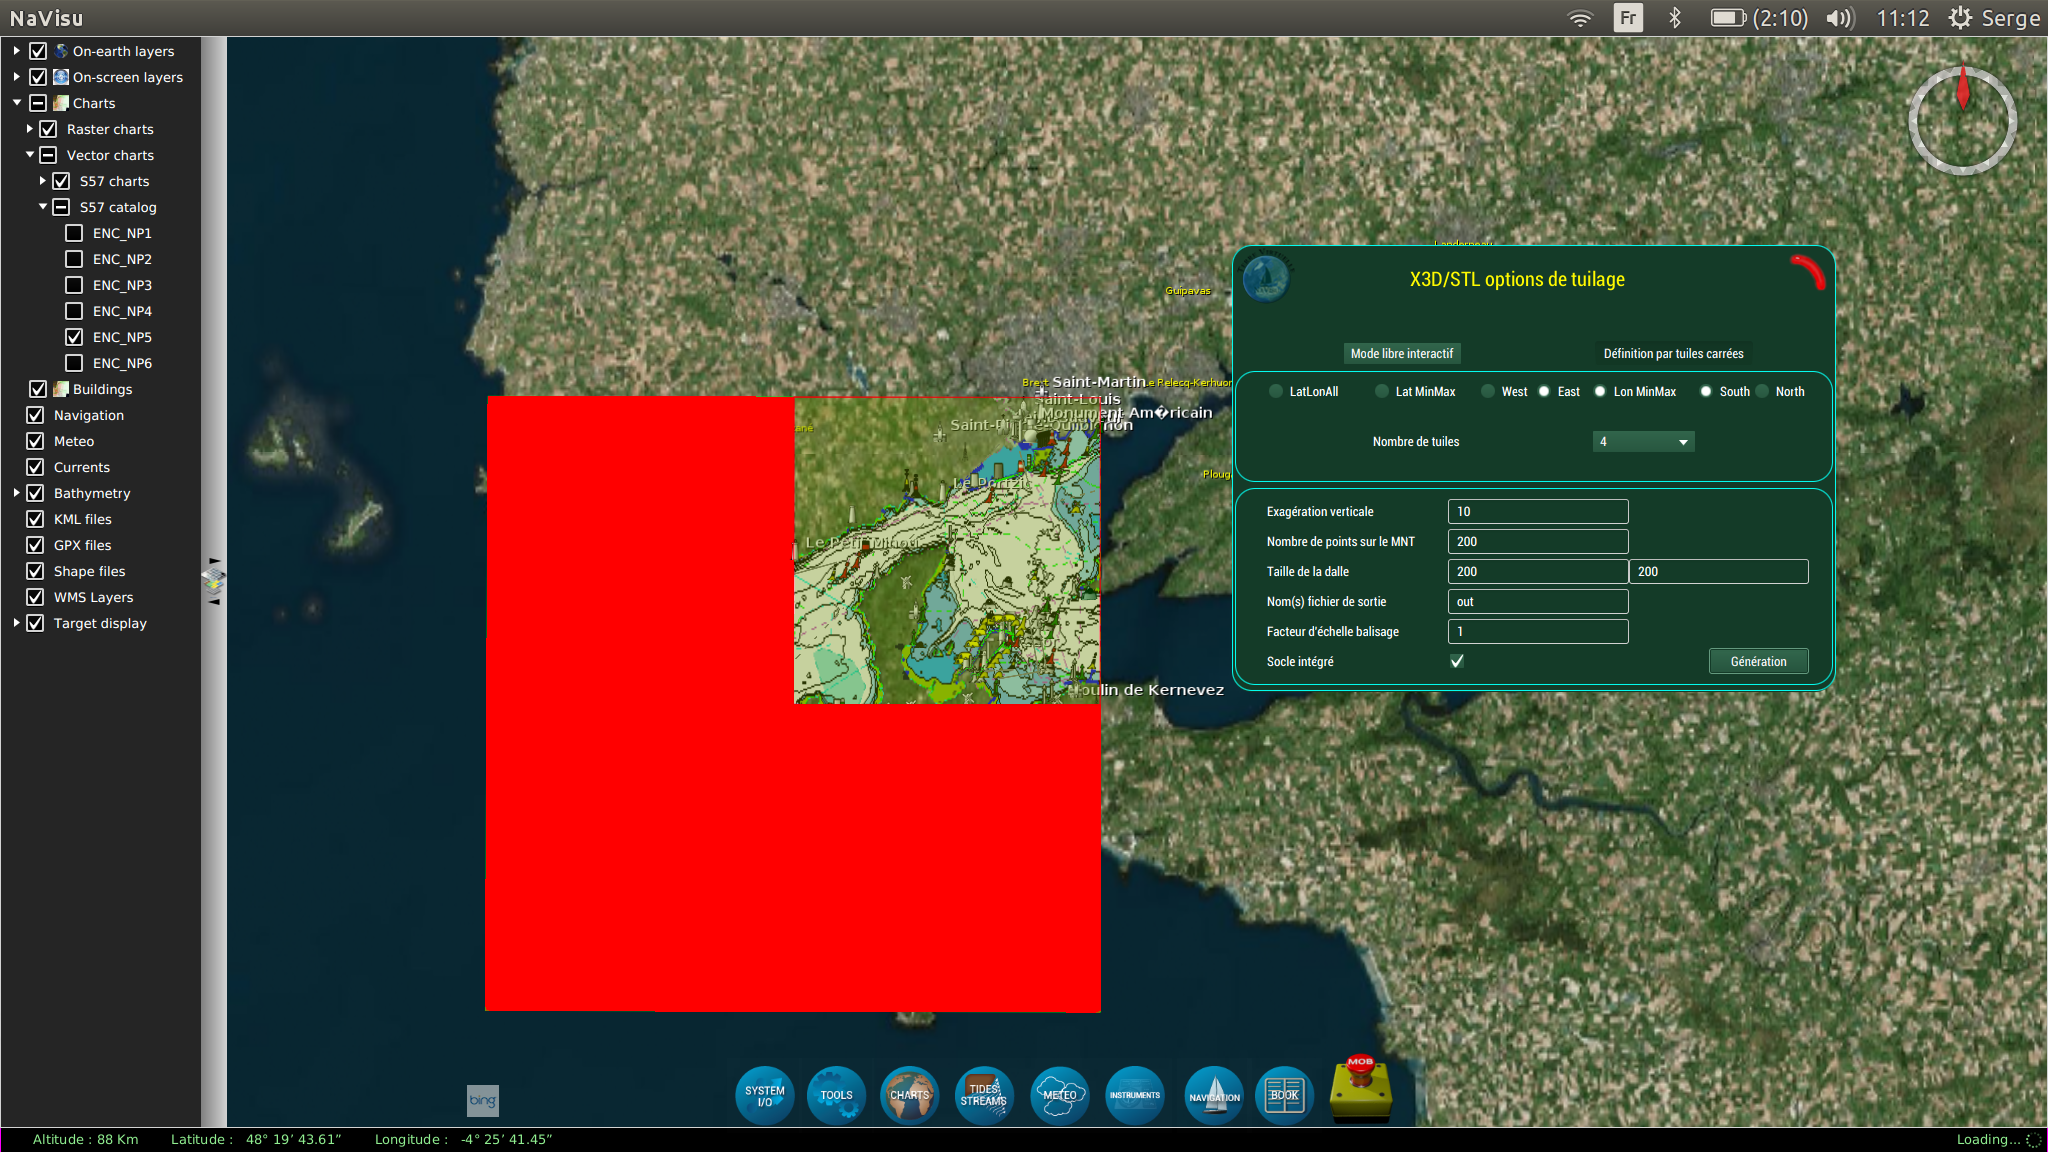
\includegraphics[width=15cm]{images/stl/generationTuiles_1.png}
	}
	\begin{figure}[ht]
		\caption{\label{sdModel}\textit{G�n�ration des tuiles}}
	\end{figure}
\end{center}
%%%%%%%%%%%%%%%%%%%%%%%%%%%%%%%%%%%%%%%%%%%%%%%%%%%%%%%%%%%%%%%%%%%%%%%
\section{Import Export des fichiers x3D}
Le format de donn�es \href{http://x3dgraphics.com/examples/X3dForWebAuthors/}{x3D} est un format {\tt xml} de description de la g�om�trie des objets et aussi de la r�activit� des objets sur le web. Nous utilisons le premier groupe de commandes. Il poss�de un ensemble de primitives : {\tt Cylinder, Box, Elevation Grid, \ldots}, ces primitives ne sont pas reconnues par les logiciels de g�n�ration STL. Elles simplifie significativement la g�n�ration de code � partir des donn�es NaVisu, aussi nous utilisons le passage par Blender, qui accepte ces donn�es en import et g�n�re pour ces objets de simples faces index�es.
%%%%%%%%%%%%%%%%%%%%%%%%%%%%%%%%%%%%%%%%%%%%%%%%%%%%%%%%%%%%%%%%%%%%%%%
\begin{center}
	\framebox[1\width]{
		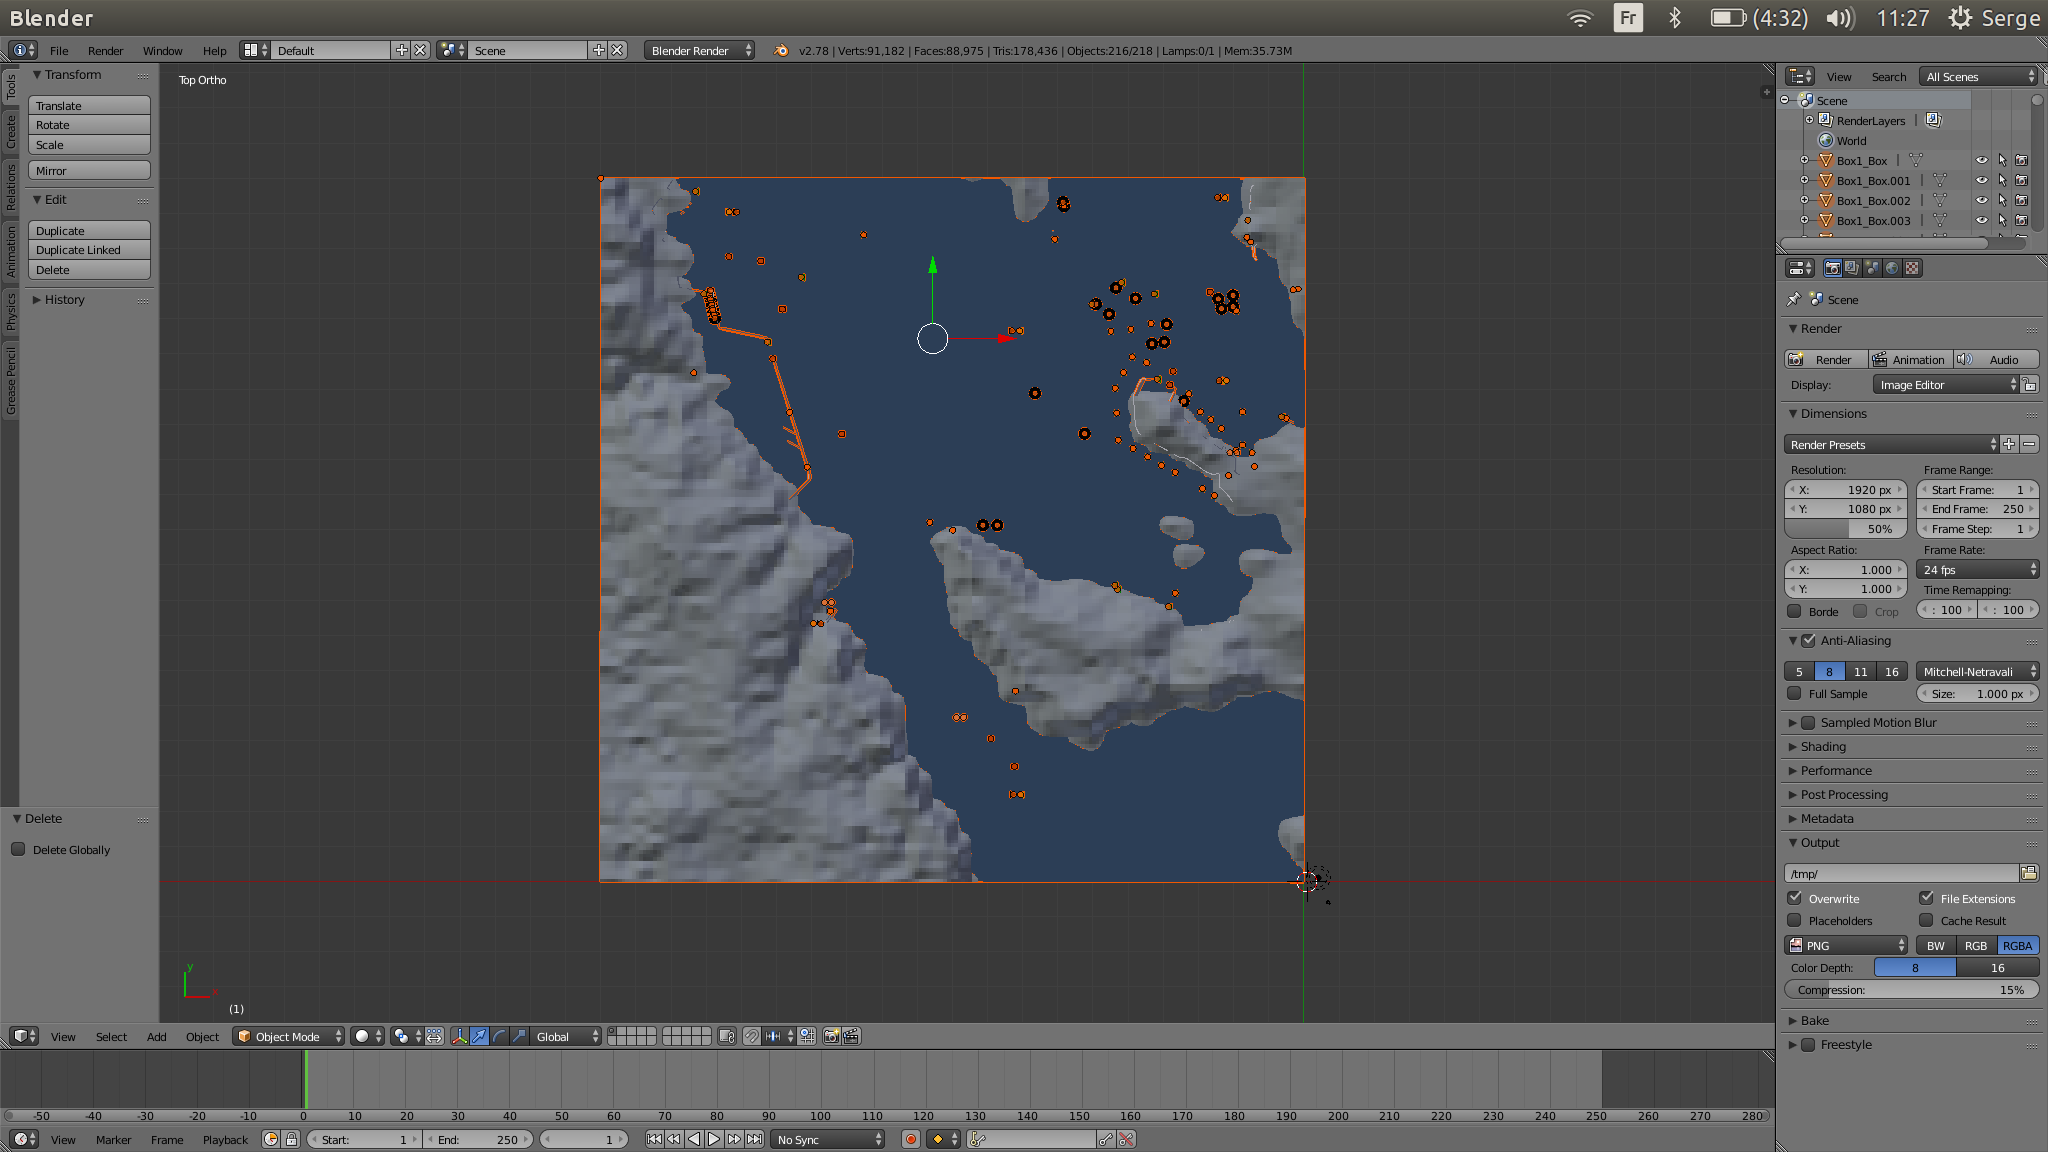
\includegraphics[width=15cm]{images/stl/blender.png}
	}
	\begin{figure}[ht]
		\caption{\label{sdModel}\textit{Import du fichier .x3d dans Blender, puis export en .x3d : g�n�ration des facettes simples.}}
	\end{figure}
\end{center}
%%%%%%%%%%%%%%%%%%%%%%%%%%%%%%%%%%%%%%%%%%%%%%%%%%%%%%%%%%%%%%%%%%%%%%%
\section{Visualisation des donn�es x3D}
Comme premi�re validation du travail, nous pouvons visualiser les donn�es x3D � l'aide de l'outil : \href{https://savage.nps.edu/X3D-Edit/#Downloads}{X3DEdit}
%%%%%%%%%%%%%%%%%%%%%%%%%%%%%%%%%%%%%%%%%%%%%%%%%%%%%%%%%%%%%%%%%%%%%%%
\begin{center}
	\framebox[1\width]{
		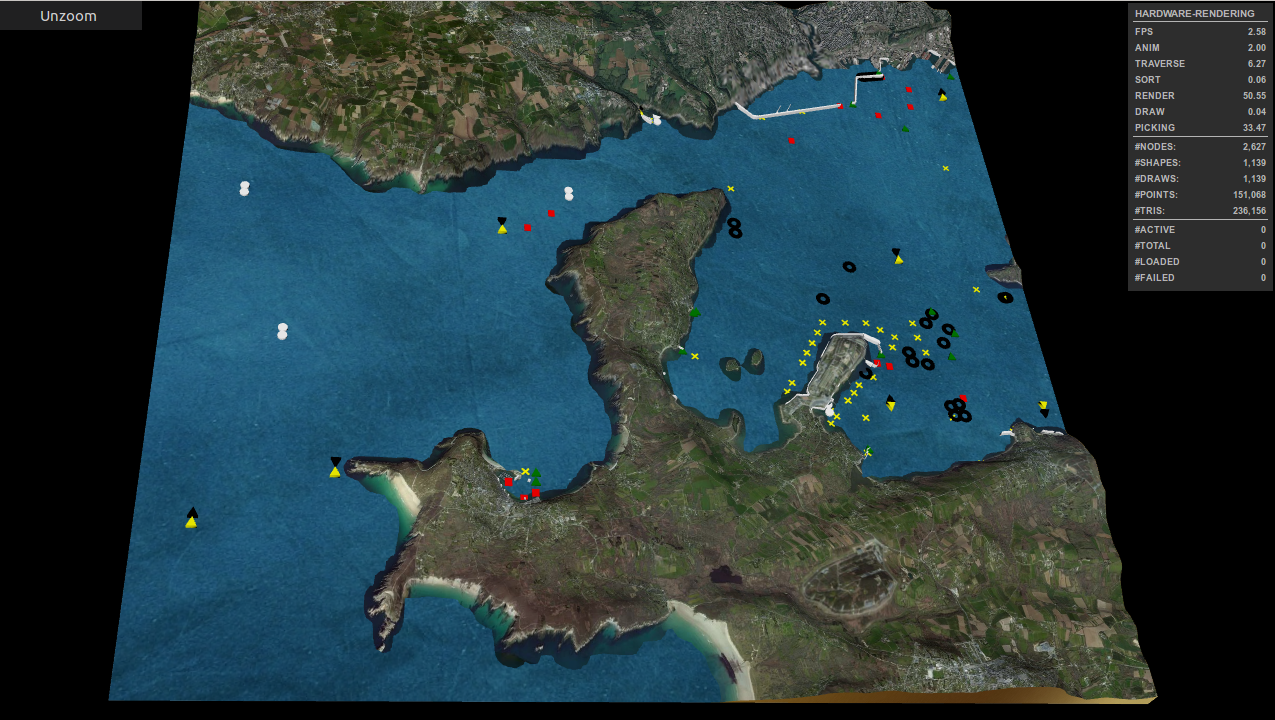
\includegraphics[width=15cm]{images/stl/x3dRade.png}
	}
	\begin{figure}[ht]
		\caption{\label{sdModel}\textit{Visualisation dans X3DEdit}}
	\end{figure}
\end{center}
%%%%%%%%%%%%%%%%%%%%%%%%%%%%%%%%%%%%%%%%%%%%%%%%%%%%%%%%%%%%%%%%%%%%%%%
\section{Logiciel de g�n�ration STL}
Nous utilisons les machines de la gamme {\bf UltiMaker}, elles peuvent �tre puilot�es par le logiciel Cura. Afin de bien valider le fichier il convient de regarder chaque couche.
%%%%%%%%%%%%%%%%%%%%%%%%%%%%%%%%%%%%%%%%%%%%%%%%%%%%%%%%%%%%%%%%%%%%%%%
\begin{center}
	\framebox[1\width]{
		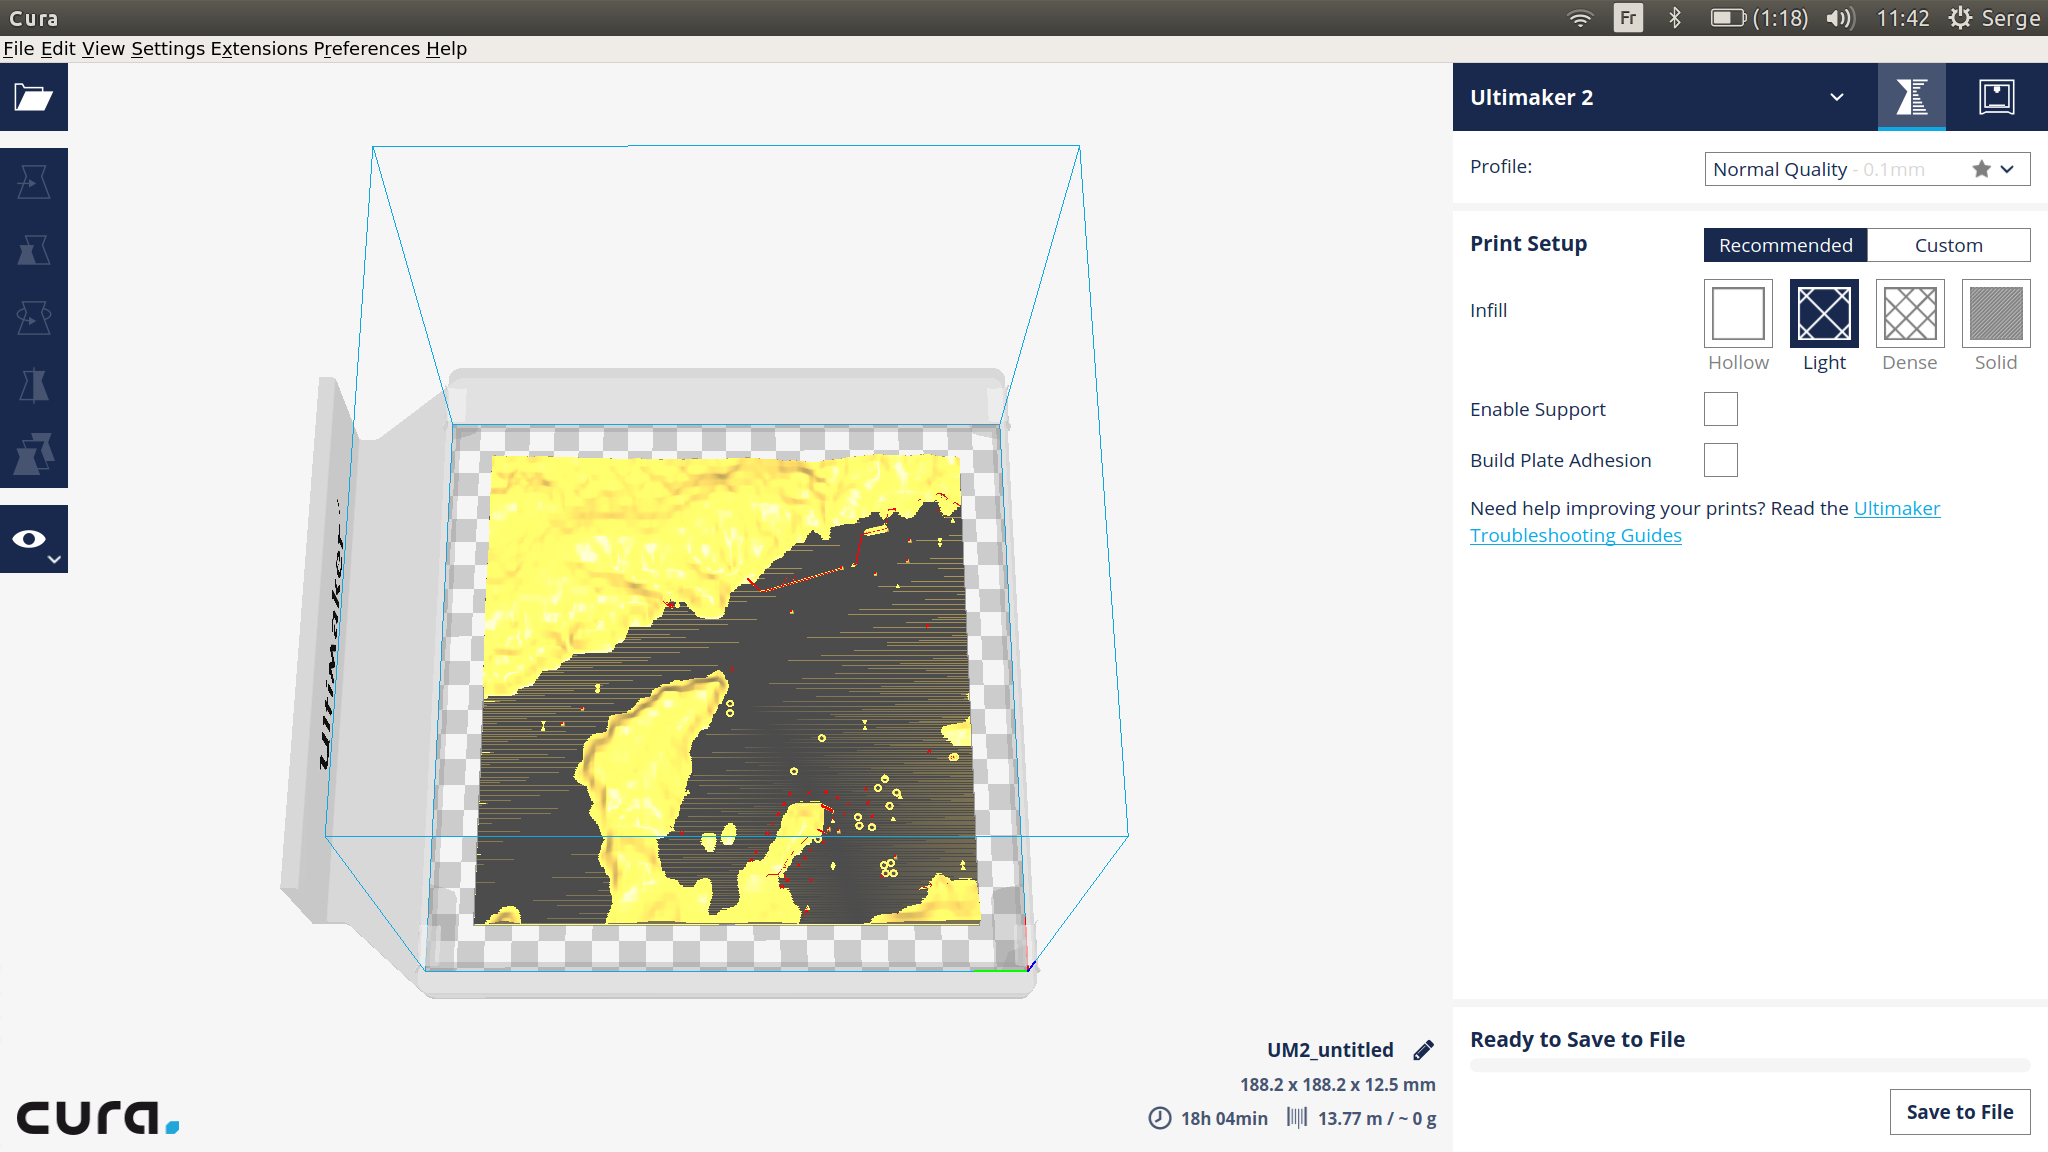
\includegraphics[width=15cm]{images/stl/cura_0.png}
	}
	\begin{figure}[ht]
		\caption{\label{sdModel}\textit{Import dans Cura}}
	\end{figure}
\end{center}
%%%%%%%%%%%%%%%%%%%%%%%%%%%%%%%%%%%%%%%%%%%%%%%%%%%%%%%%%%%%%%%%%%%%%%%
%%%%%%%%%%%%%%%%%%%%%%%%%%%%%%%%%%%%%%%%%%%%%%%%%%%%%%%%%%%%%%%%%%%%%%%
\begin{center}
	\framebox[1\width]{
		\includegraphics[width=15cm]{images/stl/cura_1.png}
	}
	\begin{figure}[ht]
		\caption{\label{sdModel}\textit{V�rification des couches dans Cura}}
	\end{figure}
\end{center}
%%%%%%%%%%%%%%%%%%%%%%%%%%%%%%%%%%%%%%%%%%%%%%%%%%%%%%%%%%%%%%%%%%%%%%%
%%%%%%%%%%%%%%%%%%%%%%%%%%%%%%%%%%%%%%%%%%%%%%%%%%%%%%%%%%%%%%%%%%%%%%%
\begin{center}
	\framebox[1\width]{
		\includegraphics[width=15cm]{images/stl/cura_2.png}
	}
	\begin{figure}[ht]
		\caption{\label{sdModel}\textit{V�rification des couches dans Cura, ici le socle.}}
	\end{figure}
\end{center}
%%%%%%%%%%%%%%%%%%%%%%%%%%%%%%%%%%%%%%%%%%%%%%%%%%%%%%%%%%%%%%%%%%%%%%%
\section{La bathym�trie}

La pr�cision du MNT de base fourni par WorldWind est suffisante pour des applications maritimes, la cartographie � partir des cartes vectorielles S57 est tr�s pr�cise, par contre la pr�cision de la bathym�trie est tr�s variable suivant les endroits du monde. Elle est insuffisante pour des applications maritimes dans nos latitudes. Pour la France, le SHOM, projet Homonim, met � la disposition du public des donn�es sous diff�rents formats. \href{http://diffusion.shom.fr/produits/bathymetrie/mnt-facade-atl-homonim.html}{MNT Bathym�trique de la fa�ade atlantique}. Le volume de ces donn�es est important et pour leur exploitation il convient de les stocker dans une base de donn�es. Nous avons fait le choix de la base PostGis. Le module {\tt navisu-stl}, utilise les modules {\tt navisu-bathymetry} pour les services de visualisation des donn�es de profondeur et le module {\tt navisu-db} pour les services de connexion aux bases de donn�es.\\
Carat�ristiques de la base de donn�es
\begin{itemize}
	\item base PostgresSQL
	\item name : BathyShomB
	\item template : postgres
	\item user : admin
	\item passwd : admin
\end{itemize}
%%%%%%%%%%%%%%%%%%%%%%%%%%%%%%%%%%%%%%%%%%%%%%%%%%%%%%%%%%%%%%%%%%%%%%%
\begin{center}
	\framebox[1\width]{
		\includegraphics[width=15cm]{images/bathy/bathy_11.png}
	}
	\begin{figure}[ht]
		\caption{\label{sdModel}\textit{Triangulation niveau 0 + bathym�trie}}
	\end{figure}
\end{center}
%%%%%%%%%%%%%%%%%%%%%%%%%%%%%%%%%%%%%%%%%%%%%%%%%%%%%%%%%%%%%%%%%%%%%%%

\chapter*{Module {\tt navisu-extensions}}
\section{La commande {\bf \tt TargetCmd}}
Dans ce document on s'attache surtout � la description de l'utilisation de cette commande et non pas � son impl�mentation.
Les {\tt TargetCmd} permettent d'interroger NaVisu sur la position d'objets de type {\tt NavigationData}, c'est � dire la plupart des objets d'une carte S57, par rapport � une position d�finie par l'utilisateur. \\
Construction d'une commande {\tt TargetCmd} cot� client : 
\begin{Verbatim}[frame=single]
Target target = new Target(new BeaconCardinal(), 48.3130, -4.6214));
Command navCmd = new Command("TargetCmd", target);
\end{Verbatim}

 %%%%%%%%%%%%%%%%%%%%%%%%%%%%%%%%%%%%%%%%%%%%%%%%%%%%% 
\begin{center}
	\framebox[1\width]{
		\includegraphics[width=19cm]{images/extension/target.png}
	}
	\begin{figure}[ht]
		\caption{\label{3}\textit{La classe {\tt Target}}}
	\end{figure}
\end{center}
%%%%%%%%%%%%%%%%%%%%%%%%%%%%%%%%%%%%%%%%%%%%%%%%%%%%%%%
Comme les autres commandes, le premier argument est le nom de la commande. Le second argument est du type {\tt Target} qui impl�mente l'interface : {\tt NavigationData}. Cet objet {\tt Target} est aussi susceptible de poss�der un objet de type {\tt NavigationData}.\\
Apr�s r�ception et traitement par NaVisu, un objet de type {\tt NavigationDataSet} sera renvoy�.
\subsection{Construction de l'objet {\tt Target} pour la requ�te}
\begin{itemize}
\item Lors de l'�mission de la requ�te, cet argument sert � d�finir le type pr�cis d'objets � cibler. On se contente alors d'utiliser un constructeur par d�faut. On peut affiner la requ�te en pr�cisant un type exact ou au contraire l'�largir en donnant une super classe.  Par exemple {\tt Buoyage} pour cibler tout type de balisage.
\end{itemize}
 %%%%%%%%%%%%%%%%%%%%%%%%%%%%%%%%%%%%%%%%%%%%%%%%%%%%% 
\begin{center}
	\framebox[1\width]{
		\includegraphics[width=18cm]{images/extension/buoyage.png}
	}
	\begin{figure}[ht]
		\caption{\label{3}\textit{Les classes {\tt Buoyage}}}
	\end{figure}
\end{center}
%%%%%%%%%%%%%%%%%%%%%%%%%%%%%%%%%%%%%%%%%%%%%%%%%%%%%%%
\begin{itemize}
\item Les deux doubles suivants d�finissent la position de l'observateur. C'est par rapport � cette position que seront cibl�s les objets dans NaVisu.
Les arguments suivants sont optionnels.
\item Un identifiant peut �tre ajout�, � l'usage du client.
\item L'argument {\tt distance} : s'il n'est pas pr�sent : le premier objet r�pondant au type demand� sera renvoy�.
S'il est pr�sent le ou les objets, r�pondant au type demand�, se trouvant dans un cercle dont le rayon est d�fini par cette distance, seront renvoy�s (l'unit� est le m�tre).
\item Si l'argument {\tt azimuth} est pr�sent, les donn�es dans un secteur {\tt azimuth $\pm 10�$} seront renvoy�es, �ventuellement filtr�es par la distance.
\end{itemize}
\subsection{Exemple de codage d'un client}
Voir un exemple : \href{https://github.com/terre-virtuelle/NaVisuClient}{https://github.com/terre-virtuelle/NaVisuClient}
\begin{itemize}
\item Initialisation du client.
\item Ouverture du canal "/navigation" sur le serveur
\item Cr�ation des requ�tes
\end{itemize}
{\small
\begin{Verbatim}[frame=single]

public void init() {
	cmdVertx = VertxFactory.newVertx();
	cmdVertx.createHttpClient().setHost("localhost")
	.setPort(9090)
	.connectWebsocket("/navigation", (WebSocket websocket) -> {
	websocket.dataHandler((Buffer data) -> {
		if (data != null) {
			response(data.toString());
		}
	});
	cmdWS = websocket;
	cmdRequest(new Target(new BeaconCardinal(), 48.3130, -4.6214)); 
	cmdRequest(new Target(new Buoyage(), 48.3130, -4.6214));
	cmdRequest(new Target(new BeaconSpecialPurpose(), 48.3130, -4.6214));
	});
}
\end{Verbatim}
}
\begin{itemize}
\item Instanciation de la commande
\item S�rialisation de l'objet commande en xml
\item Envoi au serveur.
\end{itemize}
{\small
\begin{Verbatim}[frame=single]

public void cmdRequest(NavigationData target) {
	Writer stringWriter = new StringWriter();
	Command navCmd = new Command("TargetCmd", target);
	try {
		ImportExportXML.exports(navCmd, stringWriter);
	} catch (JAXBException ex) {
	Logger.getLogger(AppTarget.class.getName()).log(Level.SEVERE, null, ex);
	}
	cmdWS.writeTextFrame(stringWriter.toString());
}

\end{Verbatim}
}
\newpage
Le r�sultat est en xml
\begin{itemize}
\item Apr�s lecture du r�sultat.
\item Traduction du r�sultat en objets.
\item R�cup�ration de la liste des NavigationData et coercition de type si n�cessaire.
\item Utilisation des donn�es.
\end{itemize}
{\small
\begin{Verbatim}[frame=single]

private void response(String resp) {

	NavigationDataSet navigationDataSet = new NavigationDataSet();
	try {
		navigationDataSet = ImportExportXML.imports(navigationDataSet,
		 new StringReader(resp));
	} catch (JAXBException ex) {
	Logger.getLogger(App.class.getName()).log(Level.SEVERE, ex.toString(), ex);
	}

	List<NavigationData> result = navigationDataSet.getNavigationDataList();
	for (NavigationData n : result) {
		Target t = (Target) n;
		System.out.print("buoy : " 
		+ ((Buoyage) t.getNavigationData()).getObjectName());
		System.out.print(" type : " 
		+ t.getNavigationData().getClass().getSimpleName());
		System.out.printf(" distance : %.2f m", t.getDistance());
		System.out.printf(" azimuth : %.2f �\n", t.getAzimuth());
	}
}

\end{Verbatim}
}
\subsection{Visualisation sur NaVisu}

En plus de renvoyer la liste des objets cibl�s, NaVisu visualise les requ�tes et les �l�ments trouv�s sur la carte. R�sultat des trois requ�tes pr�c�dentes :

\begin{Verbatim}[frame=single]
cmdRequest(new Target(new BeaconCardinal(), 48.3130, -4.6214)); 
cmdRequest(new Target(new Buoyage(), 48.3130, -4.6214));
cmdRequest(new Target(new BeaconSpecialPurpose(), 48.3130, -4.6214));
\end{Verbatim}
 %%%%%%%%%%%%%%%%%%%%%%%%%%%%%%%%%%%%%%%%%%%%%%%%%%%%% 
\begin{center}
	\framebox[1\width]{
		\includegraphics[width=19cm]{images/extension/targets.png}
	}
	\begin{figure}[ht]
		\caption{\label{3}\textit{Ciblage des bou�es dans NaVisu, plusieurs crit�res de choix d'objets, sans param�tres de distance}}
	\end{figure}
\end{center}
%%%%%%%%%%%%%%%%%%%%%%%%%%%%%%%%%%%%%%%%%%%%%%%%%%%%%%%
 %%%%%%%%%%%%%%%%%%%%%%%%%%%%%%%%%%%%%%%%%%%%%%%%%%%%% 
\begin{center}
	\framebox[1\width]{
		\includegraphics[width=19cm]{images/extension/targets_1.png}
	}
	\begin{figure}[ht]
		\caption{\label{3}\textit{Ciblage des bou�es dans NaVisu avec une distance de 6000 m}}
	\end{figure}
\end{center}
%%%%%%%%%%%%%%%%%%%%%%%%%%%%%%%%%%%%%%%%%%%%%%%%%%%%%%%


	\newpage
	\label{fin}
	
	% ------------------------------------------------------------------------------
\end{document}
